\documentclass[twoside]{book}

% Packages required by doxygen
\usepackage{fixltx2e}
\usepackage{calc}
\usepackage{doxygen}
\usepackage[export]{adjustbox} % also loads graphicx
\usepackage{graphicx}
\usepackage[utf8]{inputenc}
\usepackage{makeidx}
\usepackage{multicol}
\usepackage{multirow}
\PassOptionsToPackage{warn}{textcomp}
\usepackage{textcomp}
\usepackage[nointegrals]{wasysym}
\usepackage[table]{xcolor}

% Font selection
\usepackage[T1]{fontenc}
\usepackage[scaled=.90]{helvet}
\usepackage{courier}
\usepackage{amssymb}
\usepackage{sectsty}
\renewcommand{\familydefault}{\sfdefault}
\allsectionsfont{%
  \fontseries{bc}\selectfont%
  \color{darkgray}%
}
\renewcommand{\DoxyLabelFont}{%
  \fontseries{bc}\selectfont%
  \color{darkgray}%
}
\newcommand{\+}{\discretionary{\mbox{\scriptsize$\hookleftarrow$}}{}{}}

% Page & text layout
\usepackage{geometry}
\geometry{%
  a4paper,%
  top=2.5cm,%
  bottom=2.5cm,%
  left=2.5cm,%
  right=2.5cm%
}
\tolerance=750
\hfuzz=15pt
\hbadness=750
\setlength{\emergencystretch}{15pt}
\setlength{\parindent}{0cm}
\setlength{\parskip}{3ex plus 2ex minus 2ex}
\makeatletter
\renewcommand{\paragraph}{%
  \@startsection{paragraph}{4}{0ex}{-1.0ex}{1.0ex}{%
    \normalfont\normalsize\bfseries\SS@parafont%
  }%
}
\renewcommand{\subparagraph}{%
  \@startsection{subparagraph}{5}{0ex}{-1.0ex}{1.0ex}{%
    \normalfont\normalsize\bfseries\SS@subparafont%
  }%
}
\makeatother

% Headers & footers
\usepackage{fancyhdr}
\pagestyle{fancyplain}
\fancyhead[LE]{\fancyplain{}{\bfseries\thepage}}
\fancyhead[CE]{\fancyplain{}{}}
\fancyhead[RE]{\fancyplain{}{\bfseries\leftmark}}
\fancyhead[LO]{\fancyplain{}{\bfseries\rightmark}}
\fancyhead[CO]{\fancyplain{}{}}
\fancyhead[RO]{\fancyplain{}{\bfseries\thepage}}
\fancyfoot[LE]{\fancyplain{}{}}
\fancyfoot[CE]{\fancyplain{}{}}
\fancyfoot[RE]{\fancyplain{}{\bfseries\scriptsize Generated by Doxygen }}
\fancyfoot[LO]{\fancyplain{}{\bfseries\scriptsize Generated by Doxygen }}
\fancyfoot[CO]{\fancyplain{}{}}
\fancyfoot[RO]{\fancyplain{}{}}
\renewcommand{\footrulewidth}{0.4pt}
\renewcommand{\chaptermark}[1]{%
  \markboth{#1}{}%
}
\renewcommand{\sectionmark}[1]{%
  \markright{\thesection\ #1}%
}

% Indices & bibliography
\usepackage{natbib}
\usepackage[titles]{tocloft}
\setcounter{tocdepth}{3}
\setcounter{secnumdepth}{5}
\makeindex

% Hyperlinks (required, but should be loaded last)
\usepackage{ifpdf}
\ifpdf
  \usepackage[pdftex,pagebackref=true]{hyperref}
\else
  \usepackage[ps2pdf,pagebackref=true]{hyperref}
\fi
\hypersetup{%
  colorlinks=true,%
  linkcolor=blue,%
  citecolor=blue,%
  unicode%
}

% Custom commands
\newcommand{\clearemptydoublepage}{%
  \newpage{\pagestyle{empty}\cleardoublepage}%
}

\usepackage{caption}
\captionsetup{labelsep=space,justification=centering,font={bf},singlelinecheck=off,skip=4pt,position=top}

%===== C O N T E N T S =====

\begin{document}

% Titlepage & ToC
\hypersetup{pageanchor=false,
             bookmarksnumbered=true,
             pdfencoding=unicode
            }
\pagenumbering{roman}
\begin{titlepage}
\vspace*{7cm}
\begin{center}%
{\Large Simple\+M\+D\+P\+Library }\\
\vspace*{1cm}
{\large Generated by Doxygen 1.8.11}\\
\end{center}
\end{titlepage}
\clearemptydoublepage
\tableofcontents
\clearemptydoublepage
\pagenumbering{arabic}
\hypersetup{pageanchor=true}

%--- Begin generated contents ---
\chapter{Class Index}
\section{Class List}
Here are the classes, structs, unions and interfaces with brief descriptions\+:\begin{DoxyCompactList}
\item\contentsline{section}{\hyperlink{structBitArray}{Bit\+Array} \\*Array of bits }{\pageref{structBitArray}}{}
\item\contentsline{section}{\hyperlink{structlink__ll}{link\+\_\+ll} \\*Doubly Linked List \hyperlink{structlink__ll}{link\+\_\+ll} }{\pageref{structlink__ll}}{}
\item\contentsline{section}{\hyperlink{structLLST}{L\+L\+ST} \\*Doubly Linked List }{\pageref{structLLST}}{}
\item\contentsline{section}{\hyperlink{structmap}{map} \\*Mapa o grid de celdas }{\pageref{structmap}}{}
\item\contentsline{section}{\hyperlink{structMDP}{M\+DP} \\*A Markov Decision Process }{\pageref{structMDP}}{}
\item\contentsline{section}{\hyperlink{structnav__spec}{nav\+\_\+spec} \\*Problem parameters }{\pageref{structnav__spec}}{}
\item\contentsline{section}{\hyperlink{structS__MDP}{S\+\_\+\+M\+DP} \\*A Markov Decision Process }{\pageref{structS__MDP}}{}
\item\contentsline{section}{\hyperlink{structSP}{SP} }{\pageref{structSP}}{}
\item\contentsline{section}{\hyperlink{structstate}{state} \\*A state of an \hyperlink{structMDP}{M\+DP} }{\pageref{structstate}}{}
\end{DoxyCompactList}

\chapter{File Index}
\section{File List}
Here is a list of all documented files with brief descriptions\+:\begin{DoxyCompactList}
\item\contentsline{section}{\hyperlink{dstruct_8c}{dstruct.\+c} \\*Data Structures Library }{\pageref{dstruct_8c}}{}
\item\contentsline{section}{\hyperlink{dstruct_8h}{dstruct.\+h} \\*Data Structures Library }{\pageref{dstruct_8h}}{}
\item\contentsline{section}{\hyperlink{dstruct__test_8c}{dstruct\+\_\+test.\+c} \\*Data Structures Library Test }{\pageref{dstruct__test_8c}}{}
\item\contentsline{section}{\hyperlink{mdp_8c}{mdp.\+c} \\*Simple \hyperlink{structMDP}{M\+DP} library }{\pageref{mdp_8c}}{}
\item\contentsline{section}{\hyperlink{mdp_8h}{mdp.\+h} \\*Simple \hyperlink{structMDP}{M\+DP} library }{\pageref{mdp_8h}}{}
\item\contentsline{section}{\hyperlink{mdpnav_8c}{mdpnav.\+c} \\*Map Navigation with M\+D\+Ps }{\pageref{mdpnav_8c}}{}
\item\contentsline{section}{{\bfseries mdpnav.\+h} }{\pageref{mdpnav_8h}}{}
\item\contentsline{section}{\hyperlink{random__example_8c}{random\+\_\+example.\+c} \\*Example with a random instance of a 3 state \hyperlink{structMDP}{M\+DP} }{\pageref{random__example_8c}}{}
\item\contentsline{section}{\hyperlink{ryn__chapter__17_8c}{ryn\+\_\+chapter\+\_\+17.\+c} \\*Simple \hyperlink{structMDP}{M\+DP} library }{\pageref{ryn__chapter__17_8c}}{}
\end{DoxyCompactList}

\chapter{Class Documentation}
\hypertarget{structBitArray}{}\section{Bit\+Array Struct Reference}
\label{structBitArray}\index{Bit\+Array@{Bit\+Array}}


Array of bits.  




{\ttfamily \#include $<$dstruct.\+h$>$}

\subsection*{Public Attributes}
\begin{DoxyCompactItemize}
\item 
unsigned long long \hyperlink{structBitArray_ac22cc26395f8a292d18ea0dff63ab3d4}{size}
\item 
unsigned char $\ast$ \hyperlink{structBitArray_a4c3ccabadad2f8371b7b12f7396d01bf}{bits}
\end{DoxyCompactItemize}


\subsection{Detailed Description}
Array of bits. 

\subsection{Member Data Documentation}
\index{Bit\+Array@{Bit\+Array}!bits@{bits}}
\index{bits@{bits}!Bit\+Array@{Bit\+Array}}
\subsubsection[{\texorpdfstring{bits}{bits}}]{\setlength{\rightskip}{0pt plus 5cm}unsigned char$\ast$ Bit\+Array\+::bits}\hypertarget{structBitArray_a4c3ccabadad2f8371b7b12f7396d01bf}{}\label{structBitArray_a4c3ccabadad2f8371b7b12f7396d01bf}
the bit storage. \index{Bit\+Array@{Bit\+Array}!size@{size}}
\index{size@{size}!Bit\+Array@{Bit\+Array}}
\subsubsection[{\texorpdfstring{size}{size}}]{\setlength{\rightskip}{0pt plus 5cm}unsigned long long Bit\+Array\+::size}\hypertarget{structBitArray_ac22cc26395f8a292d18ea0dff63ab3d4}{}\label{structBitArray_ac22cc26395f8a292d18ea0dff63ab3d4}
the number of bits. 

The documentation for this struct was generated from the following file\+:\begin{DoxyCompactItemize}
\item 
\hyperlink{dstruct_8h}{dstruct.\+h}\end{DoxyCompactItemize}

\hypertarget{structlink__ll}{}\section{link\+\_\+ll Struct Reference}
\label{structlink__ll}\index{link\+\_\+ll@{link\+\_\+ll}}


Doubly Linked List \hyperlink{structlink__ll}{link\+\_\+ll}.  




{\ttfamily \#include $<$dstruct.\+h$>$}



Collaboration diagram for link\+\_\+ll\+:\nopagebreak
\begin{figure}[H]
\begin{center}
\leavevmode
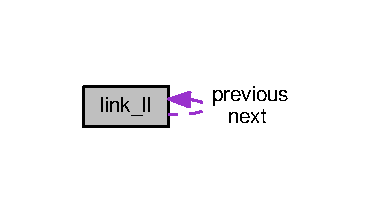
\includegraphics[width=179pt]{structlink__ll__coll__graph}
\end{center}
\end{figure}
\subsection*{Public Attributes}
\begin{DoxyCompactItemize}
\item 
void $\ast$ \hyperlink{structlink__ll_ae86aee74bb21358f58a36f9d75b04ecb}{data}
\item 
\hyperlink{structlink__ll}{link\+\_\+ll} $\ast$ \hyperlink{structlink__ll_a017a3db913bb97caa35e7c4b2be88651}{next}
\item 
struct \hyperlink{structlink__ll}{link\+\_\+ll} $\ast$ \hyperlink{structlink__ll_a48b96c80d57fcaf97793ae54d02daa49}{previous}
\end{DoxyCompactItemize}


\subsection{Detailed Description}
Doubly Linked List \hyperlink{structlink__ll}{link\+\_\+ll}. 

\subsection{Member Data Documentation}
\index{link\+\_\+ll@{link\+\_\+ll}!data@{data}}
\index{data@{data}!link\+\_\+ll@{link\+\_\+ll}}
\subsubsection[{\texorpdfstring{data}{data}}]{\setlength{\rightskip}{0pt plus 5cm}void$\ast$ link\+\_\+ll\+::data}\hypertarget{structlink__ll_ae86aee74bb21358f58a36f9d75b04ecb}{}\label{structlink__ll_ae86aee74bb21358f58a36f9d75b04ecb}
pointer to the data element. \index{link\+\_\+ll@{link\+\_\+ll}!next@{next}}
\index{next@{next}!link\+\_\+ll@{link\+\_\+ll}}
\subsubsection[{\texorpdfstring{next}{next}}]{\setlength{\rightskip}{0pt plus 5cm}{\bf link\+\_\+ll}$\ast$ link\+\_\+ll\+::next}\hypertarget{structlink__ll_a017a3db913bb97caa35e7c4b2be88651}{}\label{structlink__ll_a017a3db913bb97caa35e7c4b2be88651}
pointer to next element in this list. \index{link\+\_\+ll@{link\+\_\+ll}!previous@{previous}}
\index{previous@{previous}!link\+\_\+ll@{link\+\_\+ll}}
\subsubsection[{\texorpdfstring{previous}{previous}}]{\setlength{\rightskip}{0pt plus 5cm}struct {\bf link\+\_\+ll}$\ast$ link\+\_\+ll\+::previous}\hypertarget{structlink__ll_a48b96c80d57fcaf97793ae54d02daa49}{}\label{structlink__ll_a48b96c80d57fcaf97793ae54d02daa49}
pointer to the previous element. 

The documentation for this struct was generated from the following file\+:\begin{DoxyCompactItemize}
\item 
\hyperlink{dstruct_8h}{dstruct.\+h}\end{DoxyCompactItemize}

\hypertarget{structLLST}{}\section{L\+L\+ST Struct Reference}
\label{structLLST}\index{L\+L\+ST@{L\+L\+ST}}


Doubly Linked List.  




{\ttfamily \#include $<$dstruct.\+h$>$}



Collaboration diagram for L\+L\+ST\+:\nopagebreak
\begin{figure}[H]
\begin{center}
\leavevmode
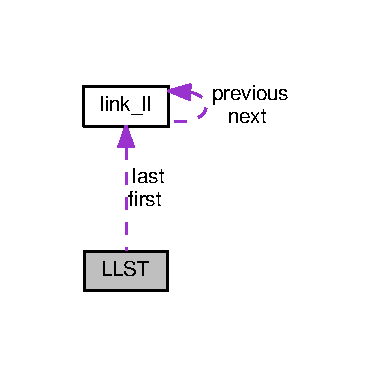
\includegraphics[width=179pt]{structLLST__coll__graph}
\end{center}
\end{figure}
\subsection*{Public Attributes}
\begin{DoxyCompactItemize}
\item 
unsigned long long \hyperlink{structLLST_a3ee1e8d7f235f4e95951006e7f52bf73}{size}
\item 
\hyperlink{structlink__ll}{link\+\_\+ll} $\ast$ \hyperlink{structLLST_a64cb4ed06a05e5d9609ee66037c2d678}{first}
\item 
\hyperlink{structlink__ll}{link\+\_\+ll} $\ast$ \hyperlink{structLLST_a036571f75af8df62f99a7db4b94d6422}{last}
\end{DoxyCompactItemize}


\subsection{Detailed Description}
Doubly Linked List. 

\subsection{Member Data Documentation}
\index{L\+L\+ST@{L\+L\+ST}!first@{first}}
\index{first@{first}!L\+L\+ST@{L\+L\+ST}}
\subsubsection[{\texorpdfstring{first}{first}}]{\setlength{\rightskip}{0pt plus 5cm}{\bf link\+\_\+ll}$\ast$ L\+L\+S\+T\+::first}\hypertarget{structLLST_a64cb4ed06a05e5d9609ee66037c2d678}{}\label{structLLST_a64cb4ed06a05e5d9609ee66037c2d678}
the first element of the list. \index{L\+L\+ST@{L\+L\+ST}!last@{last}}
\index{last@{last}!L\+L\+ST@{L\+L\+ST}}
\subsubsection[{\texorpdfstring{last}{last}}]{\setlength{\rightskip}{0pt plus 5cm}{\bf link\+\_\+ll}$\ast$ L\+L\+S\+T\+::last}\hypertarget{structLLST_a036571f75af8df62f99a7db4b94d6422}{}\label{structLLST_a036571f75af8df62f99a7db4b94d6422}
the last element of the list. \index{L\+L\+ST@{L\+L\+ST}!size@{size}}
\index{size@{size}!L\+L\+ST@{L\+L\+ST}}
\subsubsection[{\texorpdfstring{size}{size}}]{\setlength{\rightskip}{0pt plus 5cm}unsigned long long L\+L\+S\+T\+::size}\hypertarget{structLLST_a3ee1e8d7f235f4e95951006e7f52bf73}{}\label{structLLST_a3ee1e8d7f235f4e95951006e7f52bf73}
the size of the list. 

The documentation for this struct was generated from the following file\+:\begin{DoxyCompactItemize}
\item 
\hyperlink{dstruct_8h}{dstruct.\+h}\end{DoxyCompactItemize}

\hypertarget{structmap}{}\section{map Struct Reference}
\label{structmap}\index{map@{map}}


Mapa o grid de celdas.  




{\ttfamily \#include $<$mdp.\+h$>$}



Collaboration diagram for map\+:\nopagebreak
\begin{figure}[H]
\begin{center}
\leavevmode
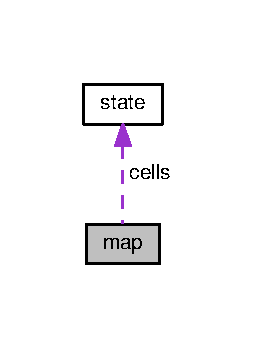
\includegraphics[width=123pt]{structmap__coll__graph}
\end{center}
\end{figure}
\subsection*{Public Attributes}
\begin{DoxyCompactItemize}
\item 
int \hyperlink{structmap_a2ee828fe96a115fe070e8ff8eea7b488}{rows}
\item 
int \hyperlink{structmap_a8519a22ad01493b189ad4ee64eb5b7dc}{columns}
\item 
\hyperlink{structstate}{state} $\ast$$\ast$ \hyperlink{structmap_a8aeb7b72916950e546c70ec3567c2e21}{cells}
\end{DoxyCompactItemize}


\subsection{Detailed Description}
Mapa o grid de celdas. 

\subsection{Member Data Documentation}
\index{map@{map}!cells@{cells}}
\index{cells@{cells}!map@{map}}
\subsubsection[{\texorpdfstring{cells}{cells}}]{\setlength{\rightskip}{0pt plus 5cm}{\bf state}$\ast$$\ast$ map\+::cells}\hypertarget{structmap_a8aeb7b72916950e546c70ec3567c2e21}{}\label{structmap_a8aeb7b72916950e546c70ec3567c2e21}
celdas del mapa \index{map@{map}!columns@{columns}}
\index{columns@{columns}!map@{map}}
\subsubsection[{\texorpdfstring{columns}{columns}}]{\setlength{\rightskip}{0pt plus 5cm}int map\+::columns}\hypertarget{structmap_a8519a22ad01493b189ad4ee64eb5b7dc}{}\label{structmap_a8519a22ad01493b189ad4ee64eb5b7dc}
number of columns \index{map@{map}!rows@{rows}}
\index{rows@{rows}!map@{map}}
\subsubsection[{\texorpdfstring{rows}{rows}}]{\setlength{\rightskip}{0pt plus 5cm}int map\+::rows}\hypertarget{structmap_a2ee828fe96a115fe070e8ff8eea7b488}{}\label{structmap_a2ee828fe96a115fe070e8ff8eea7b488}
number of rows 

The documentation for this struct was generated from the following file\+:\begin{DoxyCompactItemize}
\item 
\hyperlink{mdp_8h}{mdp.\+h}\end{DoxyCompactItemize}

\hypertarget{structMDP}{}\section{M\+DP Struct Reference}
\label{structMDP}\index{M\+DP@{M\+DP}}


A Markov Decision Process.  




{\ttfamily \#include $<$mdp.\+h$>$}

\subsection*{Public Attributes}
\begin{DoxyCompactItemize}
\item 
int \hyperlink{structMDP_aa735fb802768fb82ff8e05eb9d99ef51}{s}
\item 
int \hyperlink{structMDP_ae25a44e2b3d9f22a4f3fd6296b3602c5}{a}
\item 
float \hyperlink{structMDP_a313e7a8dc1cb9a04af91936c9daf2c62}{gamma}
\item 
float $\ast$$\ast$$\ast$ \hyperlink{structMDP_a395623fbc3e1cc9190c5acbfe4471462}{P}
\item 
unsigned char $\ast$ \hyperlink{structMDP_a70ae114113478796bd398bca88f32aa1}{t}
\item 
float $\ast$ \hyperlink{structMDP_a8335e6f1093b7551784a41cc902ef9c8}{r}
\item 
float $\ast$ \hyperlink{structMDP_ade484756ff98adafbc4c5ebbd2668b2d}{v}
\item 
int $\ast$ \hyperlink{structMDP_aeba26ff8087d7dc83fda5bd779965928}{pi}
\end{DoxyCompactItemize}


\subsection{Detailed Description}
A Markov Decision Process. 

Structure containing all parameters, infinite horizon expected rewards and optimal policy. 

\subsection{Member Data Documentation}
\index{M\+DP@{M\+DP}!a@{a}}
\index{a@{a}!M\+DP@{M\+DP}}
\subsubsection[{\texorpdfstring{a}{a}}]{\setlength{\rightskip}{0pt plus 5cm}int M\+D\+P\+::a}\hypertarget{structMDP_ae25a44e2b3d9f22a4f3fd6296b3602c5}{}\label{structMDP_ae25a44e2b3d9f22a4f3fd6296b3602c5}
number of actions \index{M\+DP@{M\+DP}!gamma@{gamma}}
\index{gamma@{gamma}!M\+DP@{M\+DP}}
\subsubsection[{\texorpdfstring{gamma}{gamma}}]{\setlength{\rightskip}{0pt plus 5cm}float M\+D\+P\+::gamma}\hypertarget{structMDP_a313e7a8dc1cb9a04af91936c9daf2c62}{}\label{structMDP_a313e7a8dc1cb9a04af91936c9daf2c62}
discount factor \index{M\+DP@{M\+DP}!P@{P}}
\index{P@{P}!M\+DP@{M\+DP}}
\subsubsection[{\texorpdfstring{P}{P}}]{\setlength{\rightskip}{0pt plus 5cm}float$\ast$$\ast$$\ast$ M\+D\+P\+::P}\hypertarget{structMDP_a395623fbc3e1cc9190c5acbfe4471462}{}\label{structMDP_a395623fbc3e1cc9190c5acbfe4471462}
transition probabilities, P(s\textquotesingle{}$\vert$s,a)(access\+: P\mbox{[}s\textquotesingle{}\mbox{]}\mbox{[}s\mbox{]}\mbox{[}a\mbox{]}) \index{M\+DP@{M\+DP}!pi@{pi}}
\index{pi@{pi}!M\+DP@{M\+DP}}
\subsubsection[{\texorpdfstring{pi}{pi}}]{\setlength{\rightskip}{0pt plus 5cm}int$\ast$ M\+D\+P\+::pi}\hypertarget{structMDP_aeba26ff8087d7dc83fda5bd779965928}{}\label{structMDP_aeba26ff8087d7dc83fda5bd779965928}
the optimal policy \index{M\+DP@{M\+DP}!r@{r}}
\index{r@{r}!M\+DP@{M\+DP}}
\subsubsection[{\texorpdfstring{r}{r}}]{\setlength{\rightskip}{0pt plus 5cm}float$\ast$ M\+D\+P\+::r}\hypertarget{structMDP_a8335e6f1093b7551784a41cc902ef9c8}{}\label{structMDP_a8335e6f1093b7551784a41cc902ef9c8}
the reward r(s) \index{M\+DP@{M\+DP}!s@{s}}
\index{s@{s}!M\+DP@{M\+DP}}
\subsubsection[{\texorpdfstring{s}{s}}]{\setlength{\rightskip}{0pt plus 5cm}int M\+D\+P\+::s}\hypertarget{structMDP_aa735fb802768fb82ff8e05eb9d99ef51}{}\label{structMDP_aa735fb802768fb82ff8e05eb9d99ef51}
number of states \index{M\+DP@{M\+DP}!t@{t}}
\index{t@{t}!M\+DP@{M\+DP}}
\subsubsection[{\texorpdfstring{t}{t}}]{\setlength{\rightskip}{0pt plus 5cm}unsigned char$\ast$ M\+D\+P\+::t}\hypertarget{structMDP_a70ae114113478796bd398bca88f32aa1}{}\label{structMDP_a70ae114113478796bd398bca88f32aa1}
terminal states \index{M\+DP@{M\+DP}!v@{v}}
\index{v@{v}!M\+DP@{M\+DP}}
\subsubsection[{\texorpdfstring{v}{v}}]{\setlength{\rightskip}{0pt plus 5cm}float$\ast$ M\+D\+P\+::v}\hypertarget{structMDP_ade484756ff98adafbc4c5ebbd2668b2d}{}\label{structMDP_ade484756ff98adafbc4c5ebbd2668b2d}
the infinite horizon expected rewards 

The documentation for this struct was generated from the following file\+:\begin{DoxyCompactItemize}
\item 
\hyperlink{mdp_8h}{mdp.\+h}\end{DoxyCompactItemize}

\hypertarget{structnav__spec}{}\section{nav\+\_\+spec Struct Reference}
\label{structnav__spec}\index{nav\+\_\+spec@{nav\+\_\+spec}}


problem parameters  




{\ttfamily \#include $<$mdpnav.\+h$>$}

\subsection*{Public Attributes}
\begin{DoxyCompactItemize}
\item 
char $\ast$ \hyperlink{structnav__spec_abb0e727791cf0839df7cea5433bff423}{input\+\_\+file}
\item 
char $\ast$ \hyperlink{structnav__spec_a9d92be20ca9352274aa021679e5c2020}{output\+\_\+file}
\item 
double \hyperlink{structnav__spec_ab195081971e36486ede5ebc50891d75b}{epsilon}
\item 
double \hyperlink{structnav__spec_a9823261754c163d75ef52c2accfe66b8}{gamma}
\end{DoxyCompactItemize}


\subsection{Detailed Description}
problem parameters 

\subsection{Member Data Documentation}
\index{nav\+\_\+spec@{nav\+\_\+spec}!epsilon@{epsilon}}
\index{epsilon@{epsilon}!nav\+\_\+spec@{nav\+\_\+spec}}
\subsubsection[{\texorpdfstring{epsilon}{epsilon}}]{\setlength{\rightskip}{0pt plus 5cm}double nav\+\_\+spec\+::epsilon}\hypertarget{structnav__spec_ab195081971e36486ede5ebc50891d75b}{}\label{structnav__spec_ab195081971e36486ede5ebc50891d75b}
maximum error \index{nav\+\_\+spec@{nav\+\_\+spec}!gamma@{gamma}}
\index{gamma@{gamma}!nav\+\_\+spec@{nav\+\_\+spec}}
\subsubsection[{\texorpdfstring{gamma}{gamma}}]{\setlength{\rightskip}{0pt plus 5cm}double nav\+\_\+spec\+::gamma}\hypertarget{structnav__spec_a9823261754c163d75ef52c2accfe66b8}{}\label{structnav__spec_a9823261754c163d75ef52c2accfe66b8}
discout factor \index{nav\+\_\+spec@{nav\+\_\+spec}!input\+\_\+file@{input\+\_\+file}}
\index{input\+\_\+file@{input\+\_\+file}!nav\+\_\+spec@{nav\+\_\+spec}}
\subsubsection[{\texorpdfstring{input\+\_\+file}{input_file}}]{\setlength{\rightskip}{0pt plus 5cm}char$\ast$ nav\+\_\+spec\+::input\+\_\+file}\hypertarget{structnav__spec_abb0e727791cf0839df7cea5433bff423}{}\label{structnav__spec_abb0e727791cf0839df7cea5433bff423}
name of the input file \index{nav\+\_\+spec@{nav\+\_\+spec}!output\+\_\+file@{output\+\_\+file}}
\index{output\+\_\+file@{output\+\_\+file}!nav\+\_\+spec@{nav\+\_\+spec}}
\subsubsection[{\texorpdfstring{output\+\_\+file}{output_file}}]{\setlength{\rightskip}{0pt plus 5cm}char$\ast$ nav\+\_\+spec\+::output\+\_\+file}\hypertarget{structnav__spec_a9d92be20ca9352274aa021679e5c2020}{}\label{structnav__spec_a9d92be20ca9352274aa021679e5c2020}
name of the output file 

The documentation for this struct was generated from the following file\+:\begin{DoxyCompactItemize}
\item 
mdpnav.\+h\end{DoxyCompactItemize}

\hypertarget{structS__MDP}{}\section{S\+\_\+\+M\+DP Struct Reference}
\label{structS__MDP}\index{S\+\_\+\+M\+DP@{S\+\_\+\+M\+DP}}


A Markov Decision Process.  




{\ttfamily \#include $<$mdp.\+h$>$}



Collaboration diagram for S\+\_\+\+M\+DP\+:\nopagebreak
\begin{figure}[H]
\begin{center}
\leavevmode
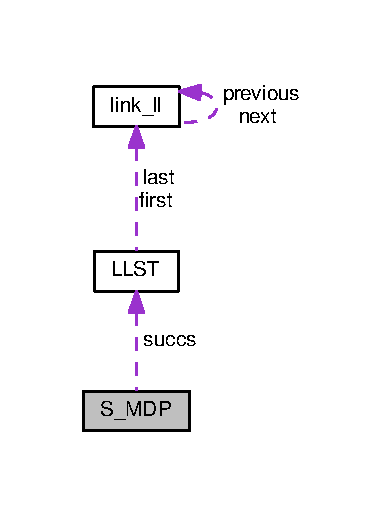
\includegraphics[width=184pt]{structS__MDP__coll__graph}
\end{center}
\end{figure}
\subsection*{Public Attributes}
\begin{DoxyCompactItemize}
\item 
int \hyperlink{structS__MDP_af679a2da7c40a40f980830cc2cbf6b77}{s}
\item 
int \hyperlink{structS__MDP_a512f18c9bed22b8a7e14be6e721499ec}{a}
\item 
double \hyperlink{structS__MDP_a973affe2889f433250f47b659609f100}{gamma}
\item 
\hyperlink{structLLST}{L\+L\+ST} $\ast$$\ast$$\ast$ \hyperlink{structS__MDP_abe58c0d8bf2759da0306273d7837f7a8}{succs}
\end{DoxyCompactItemize}


\subsection{Detailed Description}
A Markov Decision Process. 

Sparse state structure containing all parameters, infinite horizon expected rewards and optimal policy. 

\subsection{Member Data Documentation}
\index{S\+\_\+\+M\+DP@{S\+\_\+\+M\+DP}!a@{a}}
\index{a@{a}!S\+\_\+\+M\+DP@{S\+\_\+\+M\+DP}}
\subsubsection[{\texorpdfstring{a}{a}}]{\setlength{\rightskip}{0pt plus 5cm}int S\+\_\+\+M\+D\+P\+::a}\hypertarget{structS__MDP_a512f18c9bed22b8a7e14be6e721499ec}{}\label{structS__MDP_a512f18c9bed22b8a7e14be6e721499ec}
number of actions \index{S\+\_\+\+M\+DP@{S\+\_\+\+M\+DP}!gamma@{gamma}}
\index{gamma@{gamma}!S\+\_\+\+M\+DP@{S\+\_\+\+M\+DP}}
\subsubsection[{\texorpdfstring{gamma}{gamma}}]{\setlength{\rightskip}{0pt plus 5cm}double S\+\_\+\+M\+D\+P\+::gamma}\hypertarget{structS__MDP_a973affe2889f433250f47b659609f100}{}\label{structS__MDP_a973affe2889f433250f47b659609f100}
discount factor \index{S\+\_\+\+M\+DP@{S\+\_\+\+M\+DP}!s@{s}}
\index{s@{s}!S\+\_\+\+M\+DP@{S\+\_\+\+M\+DP}}
\subsubsection[{\texorpdfstring{s}{s}}]{\setlength{\rightskip}{0pt plus 5cm}int S\+\_\+\+M\+D\+P\+::s}\hypertarget{structS__MDP_af679a2da7c40a40f980830cc2cbf6b77}{}\label{structS__MDP_af679a2da7c40a40f980830cc2cbf6b77}
number of states \index{S\+\_\+\+M\+DP@{S\+\_\+\+M\+DP}!succs@{succs}}
\index{succs@{succs}!S\+\_\+\+M\+DP@{S\+\_\+\+M\+DP}}
\subsubsection[{\texorpdfstring{succs}{succs}}]{\setlength{\rightskip}{0pt plus 5cm}{\bf L\+L\+ST}$\ast$$\ast$$\ast$ S\+\_\+\+M\+D\+P\+::succs}\hypertarget{structS__MDP_abe58c0d8bf2759da0306273d7837f7a8}{}\label{structS__MDP_abe58c0d8bf2759da0306273d7837f7a8}
array of array of list of successor states. \mbox{[}s\mbox{]}\mbox{[}a\mbox{]} 

The documentation for this struct was generated from the following file\+:\begin{DoxyCompactItemize}
\item 
\hyperlink{mdp_8h}{mdp.\+h}\end{DoxyCompactItemize}

\hypertarget{structSP}{}\section{SP Struct Reference}
\label{structSP}\index{SP@{SP}}


{\ttfamily \#include $<$mdp.\+h$>$}



Collaboration diagram for SP\+:\nopagebreak
\begin{figure}[H]
\begin{center}
\leavevmode
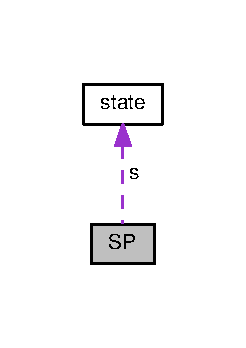
\includegraphics[width=118pt]{structSP__coll__graph}
\end{center}
\end{figure}
\subsection*{Public Attributes}
\begin{DoxyCompactItemize}
\item 
\hyperlink{structstate}{state} $\ast$ \hyperlink{structSP_a8bf41ff3d3a30c4f6f078507c176f85f}{s}
\item 
double \hyperlink{structSP_a0c560f674a6adbae23d600147c999aa5}{prob}
\end{DoxyCompactItemize}


\subsection{Detailed Description}
Next state and its probability 

\subsection{Member Data Documentation}
\index{SP@{SP}!prob@{prob}}
\index{prob@{prob}!SP@{SP}}
\subsubsection[{\texorpdfstring{prob}{prob}}]{\setlength{\rightskip}{0pt plus 5cm}double S\+P\+::prob}\hypertarget{structSP_a0c560f674a6adbae23d600147c999aa5}{}\label{structSP_a0c560f674a6adbae23d600147c999aa5}
probability of reaching the state \index{SP@{SP}!s@{s}}
\index{s@{s}!SP@{SP}}
\subsubsection[{\texorpdfstring{s}{s}}]{\setlength{\rightskip}{0pt plus 5cm}{\bf state}$\ast$ S\+P\+::s}\hypertarget{structSP_a8bf41ff3d3a30c4f6f078507c176f85f}{}\label{structSP_a8bf41ff3d3a30c4f6f078507c176f85f}
next state 

The documentation for this struct was generated from the following file\+:\begin{DoxyCompactItemize}
\item 
\hyperlink{mdp_8h}{mdp.\+h}\end{DoxyCompactItemize}

\hypertarget{structstate}{}\section{state Struct Reference}
\label{structstate}\index{state@{state}}


A state of an \hyperlink{structMDP}{M\+DP}.  




{\ttfamily \#include $<$mdp.\+h$>$}

\subsection*{Public Attributes}
\begin{DoxyCompactItemize}
\item 
int \hyperlink{structstate_a3710ff75625cc669e86b54029bb944bb}{index}
\item 
int \hyperlink{structstate_a8f960cbbf1b94dee7dc6cf2fe3b5c4c4}{type}
\item 
double \hyperlink{structstate_a85824245323f64d592c3aa55a409552b}{reward}
\item 
double \hyperlink{structstate_ac3c8aa16b56a2a479a78906a4f730786}{v}
\item 
int {\bfseries pi}\hypertarget{structstate_a4ef7ae44501808f1bffaa3290ed74ee7}{}\label{structstate_a4ef7ae44501808f1bffaa3290ed74ee7}

\end{DoxyCompactItemize}


\subsection{Detailed Description}
A state of an \hyperlink{structMDP}{M\+DP}. 

\subsection{Member Data Documentation}
\index{state@{state}!index@{index}}
\index{index@{index}!state@{state}}
\subsubsection[{\texorpdfstring{index}{index}}]{\setlength{\rightskip}{0pt plus 5cm}int state\+::index}\hypertarget{structstate_a3710ff75625cc669e86b54029bb944bb}{}\label{structstate_a3710ff75625cc669e86b54029bb944bb}
absolute index of the state \index{state@{state}!reward@{reward}}
\index{reward@{reward}!state@{state}}
\subsubsection[{\texorpdfstring{reward}{reward}}]{\setlength{\rightskip}{0pt plus 5cm}double state\+::reward}\hypertarget{structstate_a85824245323f64d592c3aa55a409552b}{}\label{structstate_a85824245323f64d592c3aa55a409552b}
the reward of the state \index{state@{state}!type@{type}}
\index{type@{type}!state@{state}}
\subsubsection[{\texorpdfstring{type}{type}}]{\setlength{\rightskip}{0pt plus 5cm}int state\+::type}\hypertarget{structstate_a8f960cbbf1b94dee7dc6cf2fe3b5c4c4}{}\label{structstate_a8f960cbbf1b94dee7dc6cf2fe3b5c4c4}
0 (not accessible), 1 (accessible) and 2 (terminal) \index{state@{state}!v@{v}}
\index{v@{v}!state@{state}}
\subsubsection[{\texorpdfstring{v}{v}}]{\setlength{\rightskip}{0pt plus 5cm}double state\+::v}\hypertarget{structstate_ac3c8aa16b56a2a479a78906a4f730786}{}\label{structstate_ac3c8aa16b56a2a479a78906a4f730786}
the infinite horizon expected reward 

The documentation for this struct was generated from the following file\+:\begin{DoxyCompactItemize}
\item 
\hyperlink{mdp_8h}{mdp.\+h}\end{DoxyCompactItemize}

\chapter{File Documentation}
\hypertarget{dstruct_8c}{}\section{dstruct.\+c File Reference}
\label{dstruct_8c}\index{dstruct.\+c@{dstruct.\+c}}


Data Structures Library.  


{\ttfamily \#include \char`\"{}dstruct.\+h\char`\"{}}\\*
{\ttfamily \#include $<$stdlib.\+h$>$}\\*
{\ttfamily \#include $<$stdio.\+h$>$}\\*
Include dependency graph for dstruct.\+c\+:\nopagebreak
\begin{figure}[H]
\begin{center}
\leavevmode
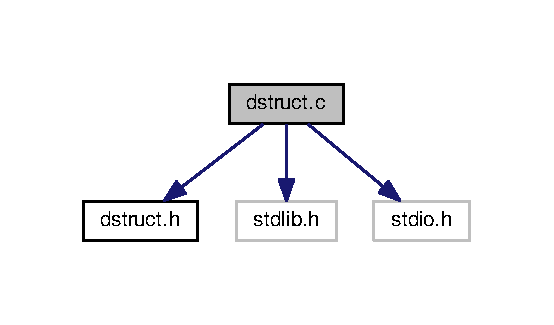
\includegraphics[width=266pt]{dstruct_8c__incl}
\end{center}
\end{figure}
\subsection*{Functions}
\begin{DoxyCompactItemize}
\item 
\hyperlink{structLLST}{L\+L\+ST} $\ast$ \hyperlink{dstruct_8c_a9997013daaafbf38572178d5a051dbc4}{empty} ()
\begin{DoxyCompactList}\small\item\em empty list \end{DoxyCompactList}\item 
void \hyperlink{dstruct_8c_a8d6b02f94753ab2fb7efa5ee5b3c0e36}{append} (\hyperlink{structLLST}{L\+L\+ST} $\ast$list, void $\ast$data)
\begin{DoxyCompactList}\small\item\em appends an elemento to the link\+\_\+lled list \end{DoxyCompactList}\item 
void \hyperlink{dstruct_8c_a12a28ff00e85a0e73366c4c0628b83d0}{join} (\hyperlink{structLLST}{L\+L\+ST} $\ast$a, \hyperlink{structLLST}{L\+L\+ST} $\ast$b)
\begin{DoxyCompactList}\small\item\em concatenates the second list in the first deleting the memory of the second \end{DoxyCompactList}\item 
\hyperlink{structLLST}{L\+L\+ST} $\ast$ \hyperlink{dstruct_8c_a3270d6a90fe0e32c69d4794980a57b94}{concat} (\hyperlink{structLLST}{L\+L\+ST} $\ast$a, \hyperlink{structLLST}{L\+L\+ST} $\ast$b)
\begin{DoxyCompactList}\small\item\em creates a new list with the concatenation of a and b \end{DoxyCompactList}\item 
\hyperlink{structlink__ll}{link\+\_\+ll} $\ast$ \hyperlink{dstruct_8c_ad0c3db380f4f51cba85896c50494b9aa}{new\+\_\+link\+\_\+ll} (void $\ast$data, \hyperlink{structlink__ll}{link\+\_\+ll} $\ast$previous, \hyperlink{structlink__ll}{link\+\_\+ll} $\ast$next)
\begin{DoxyCompactList}\small\item\em creates the new \hyperlink{structlink__ll}{link\+\_\+ll} with the provided parameters \end{DoxyCompactList}\item 
\hyperlink{structLLST}{L\+L\+ST} $\ast$ \hyperlink{dstruct_8c_a867d5f07126b1c5e69a61d3e876c95e6}{copy} (\hyperlink{structLLST}{L\+L\+ST} $\ast$list)
\begin{DoxyCompactList}\small\item\em creates a shallow copy of the provided list \end{DoxyCompactList}\item 
void $\ast$ \hyperlink{dstruct_8c_a128ec82d7f984252abce87076664ffa5}{head} (\hyperlink{structLLST}{L\+L\+ST} $\ast$list)
\begin{DoxyCompactList}\small\item\em extracts the first element of the list (head) \end{DoxyCompactList}\item 
void \hyperlink{dstruct_8c_a9eab307b1cc708a1f6cad34a968aa2ff}{free\+\_\+\+L\+L\+ST} (\hyperlink{structLLST}{L\+L\+ST} $\ast$list)
\begin{DoxyCompactList}\small\item\em releses the memory of the list and its elements but not of the contents of the list \end{DoxyCompactList}\item 
void \hyperlink{dstruct_8c_a423c3f14ff7c6ff26e1504faf52a413c}{free\+\_\+data\+\_\+\+L\+L\+ST} (\hyperlink{structLLST}{L\+L\+ST} $\ast$list)
\begin{DoxyCompactList}\small\item\em releases the memory of all data allocated in the elements of the list \end{DoxyCompactList}\item 
\hyperlink{structBitArray}{Bit\+Array} $\ast$ \hyperlink{dstruct_8c_a41a59de89889d77d52bed8d3713fc01e}{new\+\_\+\+Bit\+Array} (unsigned long long n)
\begin{DoxyCompactList}\small\item\em creates a new Array of bits of the given size the array will be initialized with ceros \end{DoxyCompactList}\item 
void \hyperlink{dstruct_8c_a774886f9daf8a36ce5aeb5e48eac8a0e}{set\+\_\+bit} (\hyperlink{structBitArray}{Bit\+Array} $\ast$array, unsigned char bit, unsigned long long pos)
\begin{DoxyCompactList}\small\item\em sets the bit at location pos \end{DoxyCompactList}\item 
unsigned char \hyperlink{dstruct_8c_ace45d8a0941ab058bc981b2da13d1114}{get\+\_\+bit} (\hyperlink{structBitArray}{Bit\+Array} $\ast$array, unsigned long long pos)
\begin{DoxyCompactList}\small\item\em extracts the bit at the given position in the \hyperlink{structBitArray}{Bit\+Array} \end{DoxyCompactList}\item 
void \hyperlink{dstruct_8c_a4911e40684950681e490f7152314e6cb}{print\+\_\+\+Bit\+Array} (\hyperlink{structBitArray}{Bit\+Array} $\ast$array)
\begin{DoxyCompactList}\small\item\em prints the contents of the bit array \end{DoxyCompactList}\item 
void \hyperlink{dstruct_8c_aa7441c7d258fbb6ce31f2f89d85ccc5c}{free\+\_\+\+Bit\+Array} (\hyperlink{structBitArray}{Bit\+Array} $\ast$array)
\begin{DoxyCompactList}\small\item\em releases the memory used by the array \end{DoxyCompactList}\end{DoxyCompactItemize}


\subsection{Detailed Description}
Data Structures Library. 

\begin{DoxyAuthor}{Author}
Stalin Muñoz Gutiérrez 
\end{DoxyAuthor}
\begin{DoxyDate}{Date}
3 March 2019 Basic Data Structures Library Implementation File 
\end{DoxyDate}


\subsection{Function Documentation}
\index{dstruct.\+c@{dstruct.\+c}!append@{append}}
\index{append@{append}!dstruct.\+c@{dstruct.\+c}}
\subsubsection[{\texorpdfstring{append(\+L\+L\+S\+T $\ast$list, void $\ast$data)}{append(LLST *list, void *data)}}]{\setlength{\rightskip}{0pt plus 5cm}void append (
\begin{DoxyParamCaption}
\item[{{\bf L\+L\+ST} $\ast$}]{list, }
\item[{void $\ast$}]{data}
\end{DoxyParamCaption}
)}\hypertarget{dstruct_8c_a8d6b02f94753ab2fb7efa5ee5b3c0e36}{}\label{dstruct_8c_a8d6b02f94753ab2fb7efa5ee5b3c0e36}


appends an elemento to the link\+\_\+lled list 


\begin{DoxyParams}{Parameters}
{\em list} & the link\+\_\+lled list \\
\hline
{\em data} & the element to append \\
\hline
\end{DoxyParams}
\index{dstruct.\+c@{dstruct.\+c}!concat@{concat}}
\index{concat@{concat}!dstruct.\+c@{dstruct.\+c}}
\subsubsection[{\texorpdfstring{concat(\+L\+L\+S\+T $\ast$a, L\+L\+S\+T $\ast$b)}{concat(LLST *a, LLST *b)}}]{\setlength{\rightskip}{0pt plus 5cm}{\bf L\+L\+ST}$\ast$ concat (
\begin{DoxyParamCaption}
\item[{{\bf L\+L\+ST} $\ast$}]{a, }
\item[{{\bf L\+L\+ST} $\ast$}]{b}
\end{DoxyParamCaption}
)}\hypertarget{dstruct_8c_a3270d6a90fe0e32c69d4794980a57b94}{}\label{dstruct_8c_a3270d6a90fe0e32c69d4794980a57b94}


creates a new list with the concatenation of a and b 


\begin{DoxyParams}{Parameters}
{\em a} & first list \\
\hline
{\em b} & second list \\
\hline
\end{DoxyParams}
\begin{DoxyReturn}{Returns}
a new list with the concatenation of the arguments 
\end{DoxyReturn}
\index{dstruct.\+c@{dstruct.\+c}!copy@{copy}}
\index{copy@{copy}!dstruct.\+c@{dstruct.\+c}}
\subsubsection[{\texorpdfstring{copy(\+L\+L\+S\+T $\ast$list)}{copy(LLST *list)}}]{\setlength{\rightskip}{0pt plus 5cm}{\bf L\+L\+ST}$\ast$ copy (
\begin{DoxyParamCaption}
\item[{{\bf L\+L\+ST} $\ast$}]{list}
\end{DoxyParamCaption}
)}\hypertarget{dstruct_8c_a867d5f07126b1c5e69a61d3e876c95e6}{}\label{dstruct_8c_a867d5f07126b1c5e69a61d3e876c95e6}


creates a shallow copy of the provided list 


\begin{DoxyParams}{Parameters}
{\em list} & the list to copy \\
\hline
\end{DoxyParams}
\begin{DoxyReturn}{Returns}
the copy 
\end{DoxyReturn}
\index{dstruct.\+c@{dstruct.\+c}!empty@{empty}}
\index{empty@{empty}!dstruct.\+c@{dstruct.\+c}}
\subsubsection[{\texorpdfstring{empty()}{empty()}}]{\setlength{\rightskip}{0pt plus 5cm}{\bf L\+L\+ST}$\ast$ empty (
\begin{DoxyParamCaption}
{}
\end{DoxyParamCaption}
)}\hypertarget{dstruct_8c_a9997013daaafbf38572178d5a051dbc4}{}\label{dstruct_8c_a9997013daaafbf38572178d5a051dbc4}


empty list 

\begin{DoxyReturn}{Returns}
a list with cero elements 
\end{DoxyReturn}
\index{dstruct.\+c@{dstruct.\+c}!free\+\_\+\+Bit\+Array@{free\+\_\+\+Bit\+Array}}
\index{free\+\_\+\+Bit\+Array@{free\+\_\+\+Bit\+Array}!dstruct.\+c@{dstruct.\+c}}
\subsubsection[{\texorpdfstring{free\+\_\+\+Bit\+Array(\+Bit\+Array $\ast$array)}{free_BitArray(BitArray *array)}}]{\setlength{\rightskip}{0pt plus 5cm}void free\+\_\+\+Bit\+Array (
\begin{DoxyParamCaption}
\item[{{\bf Bit\+Array} $\ast$}]{array}
\end{DoxyParamCaption}
)}\hypertarget{dstruct_8c_aa7441c7d258fbb6ce31f2f89d85ccc5c}{}\label{dstruct_8c_aa7441c7d258fbb6ce31f2f89d85ccc5c}


releases the memory used by the array 


\begin{DoxyParams}{Parameters}
{\em array} & the array to release \\
\hline
\end{DoxyParams}
\index{dstruct.\+c@{dstruct.\+c}!free\+\_\+data\+\_\+\+L\+L\+ST@{free\+\_\+data\+\_\+\+L\+L\+ST}}
\index{free\+\_\+data\+\_\+\+L\+L\+ST@{free\+\_\+data\+\_\+\+L\+L\+ST}!dstruct.\+c@{dstruct.\+c}}
\subsubsection[{\texorpdfstring{free\+\_\+data\+\_\+\+L\+L\+S\+T(\+L\+L\+S\+T $\ast$list)}{free_data_LLST(LLST *list)}}]{\setlength{\rightskip}{0pt plus 5cm}void free\+\_\+data\+\_\+\+L\+L\+ST (
\begin{DoxyParamCaption}
\item[{{\bf L\+L\+ST} $\ast$}]{list}
\end{DoxyParamCaption}
)}\hypertarget{dstruct_8c_a423c3f14ff7c6ff26e1504faf52a413c}{}\label{dstruct_8c_a423c3f14ff7c6ff26e1504faf52a413c}


releases the memory of all data allocated in the elements of the list 


\begin{DoxyParams}{Parameters}
{\em list} & the list containing the data \\
\hline
\end{DoxyParams}
\index{dstruct.\+c@{dstruct.\+c}!free\+\_\+\+L\+L\+ST@{free\+\_\+\+L\+L\+ST}}
\index{free\+\_\+\+L\+L\+ST@{free\+\_\+\+L\+L\+ST}!dstruct.\+c@{dstruct.\+c}}
\subsubsection[{\texorpdfstring{free\+\_\+\+L\+L\+S\+T(\+L\+L\+S\+T $\ast$list)}{free_LLST(LLST *list)}}]{\setlength{\rightskip}{0pt plus 5cm}void free\+\_\+\+L\+L\+ST (
\begin{DoxyParamCaption}
\item[{{\bf L\+L\+ST} $\ast$}]{list}
\end{DoxyParamCaption}
)}\hypertarget{dstruct_8c_a9eab307b1cc708a1f6cad34a968aa2ff}{}\label{dstruct_8c_a9eab307b1cc708a1f6cad34a968aa2ff}


releses the memory of the list and its elements but not of the contents of the list 


\begin{DoxyParams}{Parameters}
{\em list} & the list to release \\
\hline
\end{DoxyParams}
\index{dstruct.\+c@{dstruct.\+c}!get\+\_\+bit@{get\+\_\+bit}}
\index{get\+\_\+bit@{get\+\_\+bit}!dstruct.\+c@{dstruct.\+c}}
\subsubsection[{\texorpdfstring{get\+\_\+bit(\+Bit\+Array $\ast$array, unsigned long long pos)}{get_bit(BitArray *array, unsigned long long pos)}}]{\setlength{\rightskip}{0pt plus 5cm}unsigned char get\+\_\+bit (
\begin{DoxyParamCaption}
\item[{{\bf Bit\+Array} $\ast$}]{array, }
\item[{unsigned long long}]{pos}
\end{DoxyParamCaption}
)}\hypertarget{dstruct_8c_ace45d8a0941ab058bc981b2da13d1114}{}\label{dstruct_8c_ace45d8a0941ab058bc981b2da13d1114}


extracts the bit at the given position in the \hyperlink{structBitArray}{Bit\+Array} 


\begin{DoxyParams}{Parameters}
{\em array} & the \hyperlink{structBitArray}{Bit\+Array} \\
\hline
{\em pos} & the location of the bit in the array \\
\hline
\end{DoxyParams}
\begin{DoxyReturn}{Returns}
the bit at the location 
\end{DoxyReturn}
\index{dstruct.\+c@{dstruct.\+c}!head@{head}}
\index{head@{head}!dstruct.\+c@{dstruct.\+c}}
\subsubsection[{\texorpdfstring{head(\+L\+L\+S\+T $\ast$list)}{head(LLST *list)}}]{\setlength{\rightskip}{0pt plus 5cm}void$\ast$ head (
\begin{DoxyParamCaption}
\item[{{\bf L\+L\+ST} $\ast$}]{list}
\end{DoxyParamCaption}
)}\hypertarget{dstruct_8c_a128ec82d7f984252abce87076664ffa5}{}\label{dstruct_8c_a128ec82d7f984252abce87076664ffa5}


extracts the first element of the list (head) 


\begin{DoxyParams}{Parameters}
{\em the} & list \\
\hline
\end{DoxyParams}
\begin{DoxyReturn}{Returns}
the pointer to the data, 
\end{DoxyReturn}
\index{dstruct.\+c@{dstruct.\+c}!join@{join}}
\index{join@{join}!dstruct.\+c@{dstruct.\+c}}
\subsubsection[{\texorpdfstring{join(\+L\+L\+S\+T $\ast$a, L\+L\+S\+T $\ast$b)}{join(LLST *a, LLST *b)}}]{\setlength{\rightskip}{0pt plus 5cm}void join (
\begin{DoxyParamCaption}
\item[{{\bf L\+L\+ST} $\ast$}]{a, }
\item[{{\bf L\+L\+ST} $\ast$}]{b}
\end{DoxyParamCaption}
)}\hypertarget{dstruct_8c_a12a28ff00e85a0e73366c4c0628b83d0}{}\label{dstruct_8c_a12a28ff00e85a0e73366c4c0628b83d0}


concatenates the second list in the first deleting the memory of the second 


\begin{DoxyParams}{Parameters}
{\em a} & the first list \\
\hline
{\em b} & the second list \\
\hline
\end{DoxyParams}
\index{dstruct.\+c@{dstruct.\+c}!new\+\_\+\+Bit\+Array@{new\+\_\+\+Bit\+Array}}
\index{new\+\_\+\+Bit\+Array@{new\+\_\+\+Bit\+Array}!dstruct.\+c@{dstruct.\+c}}
\subsubsection[{\texorpdfstring{new\+\_\+\+Bit\+Array(unsigned long long n)}{new_BitArray(unsigned long long n)}}]{\setlength{\rightskip}{0pt plus 5cm}{\bf Bit\+Array}$\ast$ new\+\_\+\+Bit\+Array (
\begin{DoxyParamCaption}
\item[{unsigned long long}]{n}
\end{DoxyParamCaption}
)}\hypertarget{dstruct_8c_a41a59de89889d77d52bed8d3713fc01e}{}\label{dstruct_8c_a41a59de89889d77d52bed8d3713fc01e}


creates a new Array of bits of the given size the array will be initialized with ceros 


\begin{DoxyParams}{Parameters}
{\em n} & the size of the array to allocate \\
\hline
\end{DoxyParams}
\begin{DoxyReturn}{Returns}
a reference to the array 
\end{DoxyReturn}
\index{dstruct.\+c@{dstruct.\+c}!new\+\_\+link\+\_\+ll@{new\+\_\+link\+\_\+ll}}
\index{new\+\_\+link\+\_\+ll@{new\+\_\+link\+\_\+ll}!dstruct.\+c@{dstruct.\+c}}
\subsubsection[{\texorpdfstring{new\+\_\+link\+\_\+ll(void $\ast$data, link\+\_\+ll $\ast$previous, link\+\_\+ll $\ast$next)}{new_link_ll(void *data, link_ll *previous, link_ll *next)}}]{\setlength{\rightskip}{0pt plus 5cm}{\bf link\+\_\+ll}$\ast$ new\+\_\+link\+\_\+ll (
\begin{DoxyParamCaption}
\item[{void $\ast$}]{data, }
\item[{{\bf link\+\_\+ll} $\ast$}]{previous, }
\item[{{\bf link\+\_\+ll} $\ast$}]{next}
\end{DoxyParamCaption}
)}\hypertarget{dstruct_8c_ad0c3db380f4f51cba85896c50494b9aa}{}\label{dstruct_8c_ad0c3db380f4f51cba85896c50494b9aa}


creates the new \hyperlink{structlink__ll}{link\+\_\+ll} with the provided parameters 


\begin{DoxyParams}{Parameters}
{\em data} & datum to store in the \hyperlink{structlink__ll}{link\+\_\+ll} \\
\hline
{\em previous} & previous \hyperlink{structlink__ll}{link\+\_\+ll} in the data structure \\
\hline
{\em next} & next \hyperlink{structlink__ll}{link\+\_\+ll} in the data structure \\
\hline
\end{DoxyParams}
\index{dstruct.\+c@{dstruct.\+c}!print\+\_\+\+Bit\+Array@{print\+\_\+\+Bit\+Array}}
\index{print\+\_\+\+Bit\+Array@{print\+\_\+\+Bit\+Array}!dstruct.\+c@{dstruct.\+c}}
\subsubsection[{\texorpdfstring{print\+\_\+\+Bit\+Array(\+Bit\+Array $\ast$array)}{print_BitArray(BitArray *array)}}]{\setlength{\rightskip}{0pt plus 5cm}void print\+\_\+\+Bit\+Array (
\begin{DoxyParamCaption}
\item[{{\bf Bit\+Array} $\ast$}]{array}
\end{DoxyParamCaption}
)}\hypertarget{dstruct_8c_a4911e40684950681e490f7152314e6cb}{}\label{dstruct_8c_a4911e40684950681e490f7152314e6cb}


prints the contents of the bit array 


\begin{DoxyParams}{Parameters}
{\em array} & the array of bits to print \\
\hline
\end{DoxyParams}
\index{dstruct.\+c@{dstruct.\+c}!set\+\_\+bit@{set\+\_\+bit}}
\index{set\+\_\+bit@{set\+\_\+bit}!dstruct.\+c@{dstruct.\+c}}
\subsubsection[{\texorpdfstring{set\+\_\+bit(\+Bit\+Array $\ast$array, unsigned char bit, unsigned long long pos)}{set_bit(BitArray *array, unsigned char bit, unsigned long long pos)}}]{\setlength{\rightskip}{0pt plus 5cm}void set\+\_\+bit (
\begin{DoxyParamCaption}
\item[{{\bf Bit\+Array} $\ast$}]{array, }
\item[{unsigned char}]{bit, }
\item[{unsigned long long}]{pos}
\end{DoxyParamCaption}
)}\hypertarget{dstruct_8c_a774886f9daf8a36ce5aeb5e48eac8a0e}{}\label{dstruct_8c_a774886f9daf8a36ce5aeb5e48eac8a0e}


sets the bit at location pos 


\begin{DoxyParams}{Parameters}
{\em array} & the \hyperlink{structBitArray}{Bit\+Array} \\
\hline
{\em bit} & the bit to set \\
\hline
{\em pos} & the location of the bit in the array \\
\hline
\end{DoxyParams}

\hypertarget{dstruct_8h}{}\section{dstruct.\+h File Reference}
\label{dstruct_8h}\index{dstruct.\+h@{dstruct.\+h}}


Data Structures Library.  


This graph shows which files directly or indirectly include this file\+:
\nopagebreak
\begin{figure}[H]
\begin{center}
\leavevmode
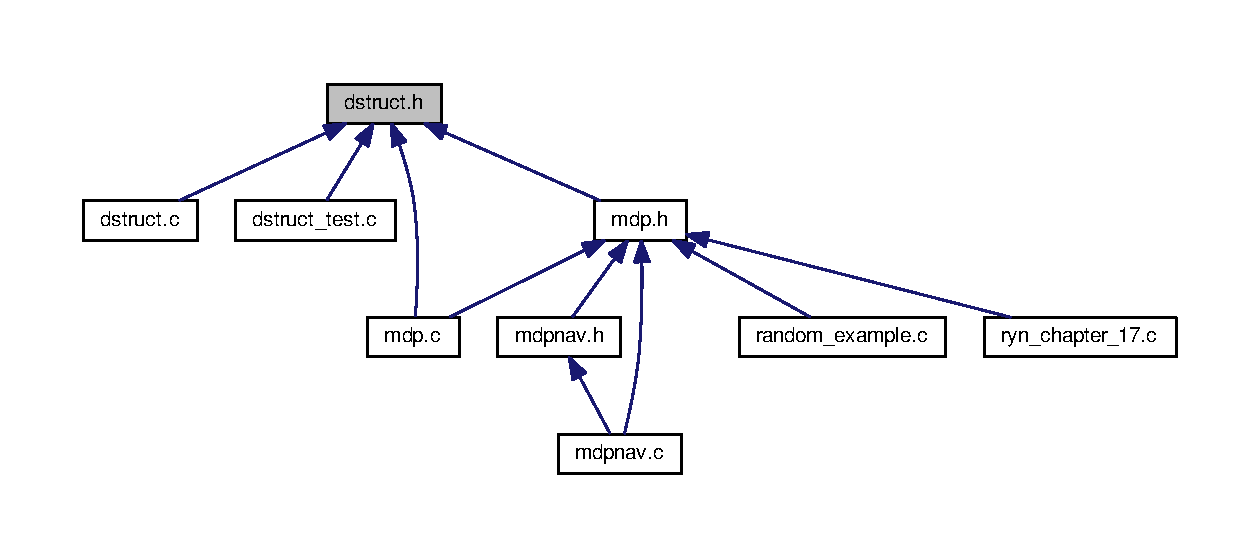
\includegraphics[width=350pt]{dstruct_8h__dep__incl}
\end{center}
\end{figure}
\subsection*{Classes}
\begin{DoxyCompactItemize}
\item 
struct \hyperlink{structlink__ll}{link\+\_\+ll}
\begin{DoxyCompactList}\small\item\em Doubly Linked List \hyperlink{structlink__ll}{link\+\_\+ll}. \end{DoxyCompactList}\item 
struct \hyperlink{structLLST}{L\+L\+ST}
\begin{DoxyCompactList}\small\item\em Doubly Linked List. \end{DoxyCompactList}\item 
struct \hyperlink{structBitArray}{Bit\+Array}
\begin{DoxyCompactList}\small\item\em Array of bits. \end{DoxyCompactList}\end{DoxyCompactItemize}
\subsection*{Macros}
\begin{DoxyCompactItemize}
\item 
\#define \hyperlink{dstruct_8h_add7ca25b1538cd6db9c19ea9e444a96a}{byteofbit}(x)~(x$>$$>$3)\hypertarget{dstruct_8h_add7ca25b1538cd6db9c19ea9e444a96a}{}\label{dstruct_8h_add7ca25b1538cd6db9c19ea9e444a96a}

\begin{DoxyCompactList}\small\item\em the byte a bit is located in a \hyperlink{structBitArray}{Bit\+Array} \end{DoxyCompactList}\item 
\#define \hyperlink{dstruct_8h_a8f125afce5fad94fc490c02893578911}{bitinbyte}(x)~(x\%8)\hypertarget{dstruct_8h_a8f125afce5fad94fc490c02893578911}{}\label{dstruct_8h_a8f125afce5fad94fc490c02893578911}

\begin{DoxyCompactList}\small\item\em the bit location in a byte \end{DoxyCompactList}\end{DoxyCompactItemize}
\subsection*{Typedefs}
\begin{DoxyCompactItemize}
\item 
typedef struct \hyperlink{structlink__ll}{link\+\_\+ll} {\bfseries link\+\_\+ll}\hypertarget{dstruct_8h_a727df6abefdea08cd30b46632842703d}{}\label{dstruct_8h_a727df6abefdea08cd30b46632842703d}

\item 
typedef struct \hyperlink{structLLST}{L\+L\+ST} \hyperlink{dstruct_8h_a99945238aaff3e71cf52d581c850b7ed}{L\+L\+ST}\hypertarget{dstruct_8h_a99945238aaff3e71cf52d581c850b7ed}{}\label{dstruct_8h_a99945238aaff3e71cf52d581c850b7ed}

\begin{DoxyCompactList}\small\item\em Doubly Linked List. \end{DoxyCompactList}\item 
typedef struct \hyperlink{structBitArray}{Bit\+Array} \hyperlink{dstruct_8h_aaa293270fd2c22825408f86d810aafb3}{Bit\+Array}\hypertarget{dstruct_8h_aaa293270fd2c22825408f86d810aafb3}{}\label{dstruct_8h_aaa293270fd2c22825408f86d810aafb3}

\begin{DoxyCompactList}\small\item\em Array of bits. \end{DoxyCompactList}\end{DoxyCompactItemize}
\subsection*{Functions}
\begin{DoxyCompactItemize}
\item 
\hyperlink{structlink__ll}{link\+\_\+ll} $\ast$ \hyperlink{dstruct_8h_ad0c3db380f4f51cba85896c50494b9aa}{new\+\_\+link\+\_\+ll} (void $\ast$data, \hyperlink{structlink__ll}{link\+\_\+ll} $\ast$previous, \hyperlink{structlink__ll}{link\+\_\+ll} $\ast$next)
\begin{DoxyCompactList}\small\item\em creates the new \hyperlink{structlink__ll}{link\+\_\+ll} with the provided parameters \end{DoxyCompactList}\item 
void \hyperlink{dstruct_8h_a8d6b02f94753ab2fb7efa5ee5b3c0e36}{append} (\hyperlink{structLLST}{L\+L\+ST} $\ast$list, void $\ast$data)
\begin{DoxyCompactList}\small\item\em appends an elemento to the link\+\_\+lled list \end{DoxyCompactList}\item 
void \hyperlink{dstruct_8h_a12a28ff00e85a0e73366c4c0628b83d0}{join} (\hyperlink{structLLST}{L\+L\+ST} $\ast$a, \hyperlink{structLLST}{L\+L\+ST} $\ast$b)
\begin{DoxyCompactList}\small\item\em concatenates the second list in the first deleting the memory of the second \end{DoxyCompactList}\item 
\hyperlink{structLLST}{L\+L\+ST} $\ast$ \hyperlink{dstruct_8h_a867d5f07126b1c5e69a61d3e876c95e6}{copy} (\hyperlink{structLLST}{L\+L\+ST} $\ast$list)
\begin{DoxyCompactList}\small\item\em creates a shallow copy of the provided list \end{DoxyCompactList}\item 
void $\ast$ \hyperlink{dstruct_8h_a128ec82d7f984252abce87076664ffa5}{head} (\hyperlink{structLLST}{L\+L\+ST} $\ast$list)
\begin{DoxyCompactList}\small\item\em extracts the first element of the list (head) \end{DoxyCompactList}\item 
\hyperlink{structLLST}{L\+L\+ST} $\ast$ \hyperlink{dstruct_8h_a9997013daaafbf38572178d5a051dbc4}{empty} ()
\begin{DoxyCompactList}\small\item\em empty list \end{DoxyCompactList}\item 
\hyperlink{structLLST}{L\+L\+ST} $\ast$ \hyperlink{dstruct_8h_a3270d6a90fe0e32c69d4794980a57b94}{concat} (\hyperlink{structLLST}{L\+L\+ST} $\ast$a, \hyperlink{structLLST}{L\+L\+ST} $\ast$b)
\begin{DoxyCompactList}\small\item\em creates a new list with the concatenation of a and b \end{DoxyCompactList}\item 
void \hyperlink{dstruct_8h_a9eab307b1cc708a1f6cad34a968aa2ff}{free\+\_\+\+L\+L\+ST} (\hyperlink{structLLST}{L\+L\+ST} $\ast$list)
\begin{DoxyCompactList}\small\item\em releses the memory of the list and its elements but not of the contents of the list \end{DoxyCompactList}\item 
void \hyperlink{dstruct_8h_a423c3f14ff7c6ff26e1504faf52a413c}{free\+\_\+data\+\_\+\+L\+L\+ST} (\hyperlink{structLLST}{L\+L\+ST} $\ast$list)
\begin{DoxyCompactList}\small\item\em releases the memory of all data allocated in the elements of the list \end{DoxyCompactList}\item 
\hyperlink{structBitArray}{Bit\+Array} $\ast$ \hyperlink{dstruct_8h_a41a59de89889d77d52bed8d3713fc01e}{new\+\_\+\+Bit\+Array} (unsigned long long n)
\begin{DoxyCompactList}\small\item\em creates a new Array of bits of the given size the array will be initialized with ceros \end{DoxyCompactList}\item 
void \hyperlink{dstruct_8h_a774886f9daf8a36ce5aeb5e48eac8a0e}{set\+\_\+bit} (\hyperlink{structBitArray}{Bit\+Array} $\ast$array, unsigned char bit, unsigned long long pos)
\begin{DoxyCompactList}\small\item\em sets the bit at location pos \end{DoxyCompactList}\item 
unsigned char \hyperlink{dstruct_8h_ace45d8a0941ab058bc981b2da13d1114}{get\+\_\+bit} (\hyperlink{structBitArray}{Bit\+Array} $\ast$array, unsigned long long pos)
\begin{DoxyCompactList}\small\item\em extracts the bit at the given position in the \hyperlink{structBitArray}{Bit\+Array} \end{DoxyCompactList}\item 
void \hyperlink{dstruct_8h_a4911e40684950681e490f7152314e6cb}{print\+\_\+\+Bit\+Array} (\hyperlink{structBitArray}{Bit\+Array} $\ast$array)
\begin{DoxyCompactList}\small\item\em prints the contents of the bit array \end{DoxyCompactList}\item 
void \hyperlink{dstruct_8h_aa7441c7d258fbb6ce31f2f89d85ccc5c}{free\+\_\+\+Bit\+Array} (\hyperlink{structBitArray}{Bit\+Array} $\ast$array)
\begin{DoxyCompactList}\small\item\em releases the memory used by the array \end{DoxyCompactList}\end{DoxyCompactItemize}


\subsection{Detailed Description}
Data Structures Library. 

\begin{DoxyAuthor}{Author}
Stalin Muñoz Gutiérrez 
\end{DoxyAuthor}
\begin{DoxyDate}{Date}
3 March 2019 Basic Data Structures Library Header File 
\end{DoxyDate}


\subsection{Function Documentation}
\index{dstruct.\+h@{dstruct.\+h}!append@{append}}
\index{append@{append}!dstruct.\+h@{dstruct.\+h}}
\subsubsection[{\texorpdfstring{append(\+L\+L\+S\+T $\ast$list, void $\ast$data)}{append(LLST *list, void *data)}}]{\setlength{\rightskip}{0pt plus 5cm}void append (
\begin{DoxyParamCaption}
\item[{{\bf L\+L\+ST} $\ast$}]{list, }
\item[{void $\ast$}]{data}
\end{DoxyParamCaption}
)}\hypertarget{dstruct_8h_a8d6b02f94753ab2fb7efa5ee5b3c0e36}{}\label{dstruct_8h_a8d6b02f94753ab2fb7efa5ee5b3c0e36}


appends an elemento to the link\+\_\+lled list 


\begin{DoxyParams}{Parameters}
{\em list} & the link\+\_\+lled list \\
\hline
{\em data} & the element to append \\
\hline
\end{DoxyParams}
\index{dstruct.\+h@{dstruct.\+h}!concat@{concat}}
\index{concat@{concat}!dstruct.\+h@{dstruct.\+h}}
\subsubsection[{\texorpdfstring{concat(\+L\+L\+S\+T $\ast$a, L\+L\+S\+T $\ast$b)}{concat(LLST *a, LLST *b)}}]{\setlength{\rightskip}{0pt plus 5cm}{\bf L\+L\+ST}$\ast$ concat (
\begin{DoxyParamCaption}
\item[{{\bf L\+L\+ST} $\ast$}]{a, }
\item[{{\bf L\+L\+ST} $\ast$}]{b}
\end{DoxyParamCaption}
)}\hypertarget{dstruct_8h_a3270d6a90fe0e32c69d4794980a57b94}{}\label{dstruct_8h_a3270d6a90fe0e32c69d4794980a57b94}


creates a new list with the concatenation of a and b 


\begin{DoxyParams}{Parameters}
{\em a} & first list \\
\hline
{\em b} & second list \\
\hline
\end{DoxyParams}
\begin{DoxyReturn}{Returns}
a new list with the concatenation of the arguments 
\end{DoxyReturn}
\index{dstruct.\+h@{dstruct.\+h}!copy@{copy}}
\index{copy@{copy}!dstruct.\+h@{dstruct.\+h}}
\subsubsection[{\texorpdfstring{copy(\+L\+L\+S\+T $\ast$list)}{copy(LLST *list)}}]{\setlength{\rightskip}{0pt plus 5cm}{\bf L\+L\+ST}$\ast$ copy (
\begin{DoxyParamCaption}
\item[{{\bf L\+L\+ST} $\ast$}]{list}
\end{DoxyParamCaption}
)}\hypertarget{dstruct_8h_a867d5f07126b1c5e69a61d3e876c95e6}{}\label{dstruct_8h_a867d5f07126b1c5e69a61d3e876c95e6}


creates a shallow copy of the provided list 


\begin{DoxyParams}{Parameters}
{\em list} & the list to copy \\
\hline
\end{DoxyParams}
\begin{DoxyReturn}{Returns}
the copy 
\end{DoxyReturn}
\index{dstruct.\+h@{dstruct.\+h}!empty@{empty}}
\index{empty@{empty}!dstruct.\+h@{dstruct.\+h}}
\subsubsection[{\texorpdfstring{empty()}{empty()}}]{\setlength{\rightskip}{0pt plus 5cm}{\bf L\+L\+ST}$\ast$ empty (
\begin{DoxyParamCaption}
{}
\end{DoxyParamCaption}
)}\hypertarget{dstruct_8h_a9997013daaafbf38572178d5a051dbc4}{}\label{dstruct_8h_a9997013daaafbf38572178d5a051dbc4}


empty list 

\begin{DoxyReturn}{Returns}
a list with cero elements 
\end{DoxyReturn}
\index{dstruct.\+h@{dstruct.\+h}!free\+\_\+\+Bit\+Array@{free\+\_\+\+Bit\+Array}}
\index{free\+\_\+\+Bit\+Array@{free\+\_\+\+Bit\+Array}!dstruct.\+h@{dstruct.\+h}}
\subsubsection[{\texorpdfstring{free\+\_\+\+Bit\+Array(\+Bit\+Array $\ast$array)}{free_BitArray(BitArray *array)}}]{\setlength{\rightskip}{0pt plus 5cm}void free\+\_\+\+Bit\+Array (
\begin{DoxyParamCaption}
\item[{{\bf Bit\+Array} $\ast$}]{array}
\end{DoxyParamCaption}
)}\hypertarget{dstruct_8h_aa7441c7d258fbb6ce31f2f89d85ccc5c}{}\label{dstruct_8h_aa7441c7d258fbb6ce31f2f89d85ccc5c}


releases the memory used by the array 


\begin{DoxyParams}{Parameters}
{\em array} & the array to release \\
\hline
\end{DoxyParams}
\index{dstruct.\+h@{dstruct.\+h}!free\+\_\+data\+\_\+\+L\+L\+ST@{free\+\_\+data\+\_\+\+L\+L\+ST}}
\index{free\+\_\+data\+\_\+\+L\+L\+ST@{free\+\_\+data\+\_\+\+L\+L\+ST}!dstruct.\+h@{dstruct.\+h}}
\subsubsection[{\texorpdfstring{free\+\_\+data\+\_\+\+L\+L\+S\+T(\+L\+L\+S\+T $\ast$list)}{free_data_LLST(LLST *list)}}]{\setlength{\rightskip}{0pt plus 5cm}void free\+\_\+data\+\_\+\+L\+L\+ST (
\begin{DoxyParamCaption}
\item[{{\bf L\+L\+ST} $\ast$}]{list}
\end{DoxyParamCaption}
)}\hypertarget{dstruct_8h_a423c3f14ff7c6ff26e1504faf52a413c}{}\label{dstruct_8h_a423c3f14ff7c6ff26e1504faf52a413c}


releases the memory of all data allocated in the elements of the list 


\begin{DoxyParams}{Parameters}
{\em list} & the list containing the data \\
\hline
\end{DoxyParams}
\index{dstruct.\+h@{dstruct.\+h}!free\+\_\+\+L\+L\+ST@{free\+\_\+\+L\+L\+ST}}
\index{free\+\_\+\+L\+L\+ST@{free\+\_\+\+L\+L\+ST}!dstruct.\+h@{dstruct.\+h}}
\subsubsection[{\texorpdfstring{free\+\_\+\+L\+L\+S\+T(\+L\+L\+S\+T $\ast$list)}{free_LLST(LLST *list)}}]{\setlength{\rightskip}{0pt plus 5cm}void free\+\_\+\+L\+L\+ST (
\begin{DoxyParamCaption}
\item[{{\bf L\+L\+ST} $\ast$}]{list}
\end{DoxyParamCaption}
)}\hypertarget{dstruct_8h_a9eab307b1cc708a1f6cad34a968aa2ff}{}\label{dstruct_8h_a9eab307b1cc708a1f6cad34a968aa2ff}


releses the memory of the list and its elements but not of the contents of the list 


\begin{DoxyParams}{Parameters}
{\em list} & the list to release \\
\hline
\end{DoxyParams}
\index{dstruct.\+h@{dstruct.\+h}!get\+\_\+bit@{get\+\_\+bit}}
\index{get\+\_\+bit@{get\+\_\+bit}!dstruct.\+h@{dstruct.\+h}}
\subsubsection[{\texorpdfstring{get\+\_\+bit(\+Bit\+Array $\ast$array, unsigned long long pos)}{get_bit(BitArray *array, unsigned long long pos)}}]{\setlength{\rightskip}{0pt plus 5cm}unsigned char get\+\_\+bit (
\begin{DoxyParamCaption}
\item[{{\bf Bit\+Array} $\ast$}]{array, }
\item[{unsigned long long}]{pos}
\end{DoxyParamCaption}
)}\hypertarget{dstruct_8h_ace45d8a0941ab058bc981b2da13d1114}{}\label{dstruct_8h_ace45d8a0941ab058bc981b2da13d1114}


extracts the bit at the given position in the \hyperlink{structBitArray}{Bit\+Array} 


\begin{DoxyParams}{Parameters}
{\em array} & the \hyperlink{structBitArray}{Bit\+Array} \\
\hline
{\em pos} & the location of the bit in the array \\
\hline
\end{DoxyParams}
\begin{DoxyReturn}{Returns}
the bit at the location 
\end{DoxyReturn}
\index{dstruct.\+h@{dstruct.\+h}!head@{head}}
\index{head@{head}!dstruct.\+h@{dstruct.\+h}}
\subsubsection[{\texorpdfstring{head(\+L\+L\+S\+T $\ast$list)}{head(LLST *list)}}]{\setlength{\rightskip}{0pt plus 5cm}void$\ast$ head (
\begin{DoxyParamCaption}
\item[{{\bf L\+L\+ST} $\ast$}]{list}
\end{DoxyParamCaption}
)}\hypertarget{dstruct_8h_a128ec82d7f984252abce87076664ffa5}{}\label{dstruct_8h_a128ec82d7f984252abce87076664ffa5}


extracts the first element of the list (head) 


\begin{DoxyParams}{Parameters}
{\em the} & list \\
\hline
\end{DoxyParams}
\begin{DoxyReturn}{Returns}
the pointer to the data, 
\end{DoxyReturn}
\index{dstruct.\+h@{dstruct.\+h}!join@{join}}
\index{join@{join}!dstruct.\+h@{dstruct.\+h}}
\subsubsection[{\texorpdfstring{join(\+L\+L\+S\+T $\ast$a, L\+L\+S\+T $\ast$b)}{join(LLST *a, LLST *b)}}]{\setlength{\rightskip}{0pt plus 5cm}void join (
\begin{DoxyParamCaption}
\item[{{\bf L\+L\+ST} $\ast$}]{a, }
\item[{{\bf L\+L\+ST} $\ast$}]{b}
\end{DoxyParamCaption}
)}\hypertarget{dstruct_8h_a12a28ff00e85a0e73366c4c0628b83d0}{}\label{dstruct_8h_a12a28ff00e85a0e73366c4c0628b83d0}


concatenates the second list in the first deleting the memory of the second 


\begin{DoxyParams}{Parameters}
{\em a} & the first list \\
\hline
{\em b} & the second list \\
\hline
\end{DoxyParams}
\index{dstruct.\+h@{dstruct.\+h}!new\+\_\+\+Bit\+Array@{new\+\_\+\+Bit\+Array}}
\index{new\+\_\+\+Bit\+Array@{new\+\_\+\+Bit\+Array}!dstruct.\+h@{dstruct.\+h}}
\subsubsection[{\texorpdfstring{new\+\_\+\+Bit\+Array(unsigned long long n)}{new_BitArray(unsigned long long n)}}]{\setlength{\rightskip}{0pt plus 5cm}{\bf Bit\+Array}$\ast$ new\+\_\+\+Bit\+Array (
\begin{DoxyParamCaption}
\item[{unsigned long long}]{n}
\end{DoxyParamCaption}
)}\hypertarget{dstruct_8h_a41a59de89889d77d52bed8d3713fc01e}{}\label{dstruct_8h_a41a59de89889d77d52bed8d3713fc01e}


creates a new Array of bits of the given size the array will be initialized with ceros 


\begin{DoxyParams}{Parameters}
{\em n} & the size of the array to allocate \\
\hline
\end{DoxyParams}
\begin{DoxyReturn}{Returns}
a reference to the array 
\end{DoxyReturn}
\index{dstruct.\+h@{dstruct.\+h}!new\+\_\+link\+\_\+ll@{new\+\_\+link\+\_\+ll}}
\index{new\+\_\+link\+\_\+ll@{new\+\_\+link\+\_\+ll}!dstruct.\+h@{dstruct.\+h}}
\subsubsection[{\texorpdfstring{new\+\_\+link\+\_\+ll(void $\ast$data, link\+\_\+ll $\ast$previous, link\+\_\+ll $\ast$next)}{new_link_ll(void *data, link_ll *previous, link_ll *next)}}]{\setlength{\rightskip}{0pt plus 5cm}{\bf link\+\_\+ll}$\ast$ new\+\_\+link\+\_\+ll (
\begin{DoxyParamCaption}
\item[{void $\ast$}]{data, }
\item[{{\bf link\+\_\+ll} $\ast$}]{previous, }
\item[{{\bf link\+\_\+ll} $\ast$}]{next}
\end{DoxyParamCaption}
)}\hypertarget{dstruct_8h_ad0c3db380f4f51cba85896c50494b9aa}{}\label{dstruct_8h_ad0c3db380f4f51cba85896c50494b9aa}


creates the new \hyperlink{structlink__ll}{link\+\_\+ll} with the provided parameters 


\begin{DoxyParams}{Parameters}
{\em data} & datum to store in the \hyperlink{structlink__ll}{link\+\_\+ll} \\
\hline
{\em previous} & previous \hyperlink{structlink__ll}{link\+\_\+ll} in the data structure \\
\hline
{\em next} & next \hyperlink{structlink__ll}{link\+\_\+ll} in the data structure \\
\hline
\end{DoxyParams}
\index{dstruct.\+h@{dstruct.\+h}!print\+\_\+\+Bit\+Array@{print\+\_\+\+Bit\+Array}}
\index{print\+\_\+\+Bit\+Array@{print\+\_\+\+Bit\+Array}!dstruct.\+h@{dstruct.\+h}}
\subsubsection[{\texorpdfstring{print\+\_\+\+Bit\+Array(\+Bit\+Array $\ast$array)}{print_BitArray(BitArray *array)}}]{\setlength{\rightskip}{0pt plus 5cm}void print\+\_\+\+Bit\+Array (
\begin{DoxyParamCaption}
\item[{{\bf Bit\+Array} $\ast$}]{array}
\end{DoxyParamCaption}
)}\hypertarget{dstruct_8h_a4911e40684950681e490f7152314e6cb}{}\label{dstruct_8h_a4911e40684950681e490f7152314e6cb}


prints the contents of the bit array 


\begin{DoxyParams}{Parameters}
{\em array} & the array of bits to print \\
\hline
\end{DoxyParams}
\index{dstruct.\+h@{dstruct.\+h}!set\+\_\+bit@{set\+\_\+bit}}
\index{set\+\_\+bit@{set\+\_\+bit}!dstruct.\+h@{dstruct.\+h}}
\subsubsection[{\texorpdfstring{set\+\_\+bit(\+Bit\+Array $\ast$array, unsigned char bit, unsigned long long pos)}{set_bit(BitArray *array, unsigned char bit, unsigned long long pos)}}]{\setlength{\rightskip}{0pt plus 5cm}void set\+\_\+bit (
\begin{DoxyParamCaption}
\item[{{\bf Bit\+Array} $\ast$}]{array, }
\item[{unsigned char}]{bit, }
\item[{unsigned long long}]{pos}
\end{DoxyParamCaption}
)}\hypertarget{dstruct_8h_a774886f9daf8a36ce5aeb5e48eac8a0e}{}\label{dstruct_8h_a774886f9daf8a36ce5aeb5e48eac8a0e}


sets the bit at location pos 


\begin{DoxyParams}{Parameters}
{\em array} & the \hyperlink{structBitArray}{Bit\+Array} \\
\hline
{\em bit} & the bit to set \\
\hline
{\em pos} & the location of the bit in the array \\
\hline
\end{DoxyParams}

\hypertarget{dstruct__test_8c}{}\section{dstruct\+\_\+test.\+c File Reference}
\label{dstruct__test_8c}\index{dstruct\+\_\+test.\+c@{dstruct\+\_\+test.\+c}}


Data Structures Library Test.  


{\ttfamily \#include \char`\"{}dstruct.\+h\char`\"{}}\\*
{\ttfamily \#include $<$stdlib.\+h$>$}\\*
{\ttfamily \#include $<$stdio.\+h$>$}\\*
Include dependency graph for dstruct\+\_\+test.\+c\+:\nopagebreak
\begin{figure}[H]
\begin{center}
\leavevmode
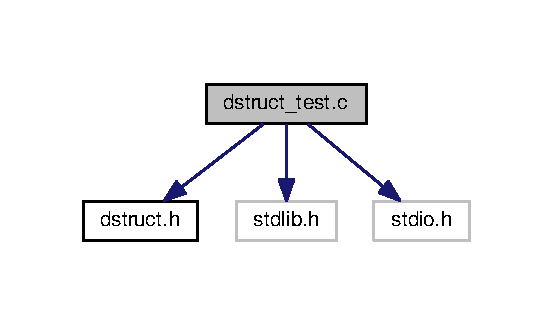
\includegraphics[width=266pt]{dstruct__test_8c__incl}
\end{center}
\end{figure}
\subsection*{Functions}
\begin{DoxyCompactItemize}
\item 
int {\bfseries main} (int argc, char $\ast$argv\mbox{[}$\,$\mbox{]})\hypertarget{dstruct__test_8c_a0ddf1224851353fc92bfbff6f499fa97}{}\label{dstruct__test_8c_a0ddf1224851353fc92bfbff6f499fa97}

\end{DoxyCompactItemize}


\subsection{Detailed Description}
Data Structures Library Test. 

\begin{DoxyAuthor}{Author}
Stalin Muñoz Gutiérrez 
\end{DoxyAuthor}
\begin{DoxyDate}{Date}
3 March 2019 Basic Data Structures Library Test File 
\end{DoxyDate}

\hypertarget{mdp_8c}{}\section{mdp.\+c File Reference}
\label{mdp_8c}\index{mdp.\+c@{mdp.\+c}}


Simple \hyperlink{structMDP}{M\+DP} library.  


{\ttfamily \#include $<$stdio.\+h$>$}\\*
{\ttfamily \#include $<$stdlib.\+h$>$}\\*
{\ttfamily \#include $<$time.\+h$>$}\\*
{\ttfamily \#include $<$float.\+h$>$}\\*
{\ttfamily \#include $<$math.\+h$>$}\\*
{\ttfamily \#include \char`\"{}mdp.\+h\char`\"{}}\\*
Include dependency graph for mdp.\+c\+:

\hypertarget{mdp_8h}{}\section{mdp.\+h File Reference}
\label{mdp_8h}\index{mdp.\+h@{mdp.\+h}}


Simple \hyperlink{structMDP}{M\+DP} library.  


{\ttfamily \#include \char`\"{}dstruct.\+h\char`\"{}}\\*
{\ttfamily \#include $<$stdlib.\+h$>$}\\*
{\ttfamily \#include $<$stdio.\+h$>$}\\*
Include dependency graph for mdp.\+h\+:\nopagebreak
\begin{figure}[H]
\begin{center}
\leavevmode
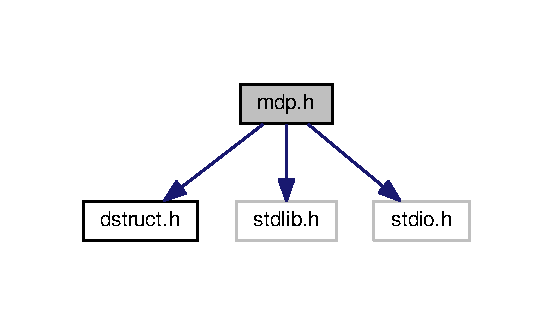
\includegraphics[width=266pt]{mdp_8h__incl}
\end{center}
\end{figure}
This graph shows which files directly or indirectly include this file\+:
\nopagebreak
\begin{figure}[H]
\begin{center}
\leavevmode
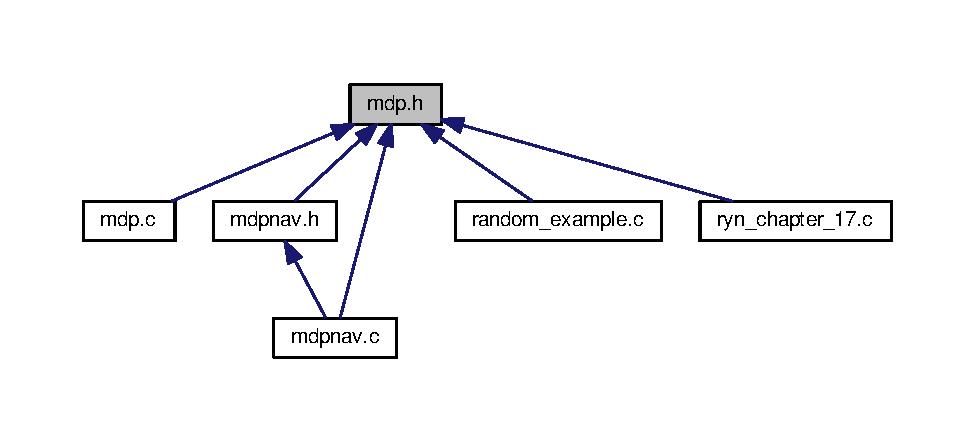
\includegraphics[width=350pt]{mdp_8h__dep__incl}
\end{center}
\end{figure}
\subsection*{Classes}
\begin{DoxyCompactItemize}
\item 
struct \hyperlink{structMDP}{M\+DP}
\begin{DoxyCompactList}\small\item\em A Markov Decision Process. \end{DoxyCompactList}\item 
struct \hyperlink{structS__MDP}{S\+\_\+\+M\+DP}
\begin{DoxyCompactList}\small\item\em A Markov Decision Process. \end{DoxyCompactList}\item 
struct \hyperlink{structstate}{state}
\begin{DoxyCompactList}\small\item\em A state of an \hyperlink{structMDP}{M\+DP}. \end{DoxyCompactList}\item 
struct \hyperlink{structSP}{SP}
\item 
struct \hyperlink{structmap}{map}
\begin{DoxyCompactList}\small\item\em Mapa o grid de celdas. \end{DoxyCompactList}\end{DoxyCompactItemize}
\subsection*{Macros}
\begin{DoxyCompactItemize}
\item 
\#define {\bfseries UP}~0\hypertarget{mdp_8h_a1965eaca47dbf3f87acdafc2208f04eb}{}\label{mdp_8h_a1965eaca47dbf3f87acdafc2208f04eb}

\item 
\#define {\bfseries R\+I\+G\+HT}~1\hypertarget{mdp_8h_a80fb826a684cf3f0d306b22aa100ddac}{}\label{mdp_8h_a80fb826a684cf3f0d306b22aa100ddac}

\item 
\#define {\bfseries D\+O\+WN}~2\hypertarget{mdp_8h_a4193cd1c8c2e6ebd0e056fa2364a663f}{}\label{mdp_8h_a4193cd1c8c2e6ebd0e056fa2364a663f}

\item 
\#define {\bfseries L\+E\+FT}~3\hypertarget{mdp_8h_a437ef08681e7210d6678427030446a54}{}\label{mdp_8h_a437ef08681e7210d6678427030446a54}

\item 
\#define {\bfseries I\+N\+A\+C\+C\+E\+SS}~0\hypertarget{mdp_8h_a09c62868b79c3f9d735d48375e62bca6}{}\label{mdp_8h_a09c62868b79c3f9d735d48375e62bca6}

\item 
\#define {\bfseries A\+C\+C\+E\+SS}~1\hypertarget{mdp_8h_a321a20f839f3d9ccd0db1dc865850dc7}{}\label{mdp_8h_a321a20f839f3d9ccd0db1dc865850dc7}

\item 
\#define {\bfseries T\+E\+R\+M\+I\+N\+AL}~2\hypertarget{mdp_8h_a5250b667cb28dd60b71e6e04e23eac37}{}\label{mdp_8h_a5250b667cb28dd60b71e6e04e23eac37}

\end{DoxyCompactItemize}
\subsection*{Functions}
\begin{DoxyCompactItemize}
\item 
\hyperlink{structMDP}{M\+DP} $\ast$ \hyperlink{mdp_8h_a548863d915fc4dc94bac432aa7d0b796}{allocate\+\_\+\+M\+DP} (int s, int a, double gamma)
\begin{DoxyCompactList}\small\item\em Allocates memory for an \hyperlink{structMDP}{M\+DP}. \end{DoxyCompactList}\item 
\hyperlink{structS__MDP}{S\+\_\+\+M\+DP} $\ast$ \hyperlink{mdp_8h_a0733bb48113b223be61b80c13fdc02aa}{allocate\+\_\+\+S\+M\+DP} (int s, int a, double gamma)
\begin{DoxyCompactList}\small\item\em Allocates memory for an Sparsed \hyperlink{structMDP}{M\+DP}. \end{DoxyCompactList}\item 
void \hyperlink{mdp_8h_a8be5eaf17931da89514166e7e6d238e6}{release\+\_\+\+S\+\_\+\+M\+DP} (\hyperlink{structS__MDP}{S\+\_\+\+M\+DP} $\ast$mdp)
\begin{DoxyCompactList}\small\item\em Releases memory for an sparsed \hyperlink{structMDP}{M\+DP}. \end{DoxyCompactList}\item 
void \hyperlink{mdp_8h_a42a1eb1c8ff10a00c6fc6313bee4f814}{release\+\_\+\+M\+DP} (\hyperlink{structMDP}{M\+DP} $\ast$mdp)
\begin{DoxyCompactList}\small\item\em Releases memory for an \hyperlink{structMDP}{M\+DP}. \end{DoxyCompactList}\item 
void \hyperlink{mdp_8h_af6d9fcae98bb545520e7244d7020dcdc}{print\+\_\+\+M\+DP} (\hyperlink{structMDP}{M\+DP} $\ast$mdp)
\begin{DoxyCompactList}\small\item\em Prints the \hyperlink{structMDP}{M\+DP} parameters. \end{DoxyCompactList}\item 
void \hyperlink{mdp_8h_a1e47a27033a991971ea6779a58585a69}{random\+\_\+\+M\+DP} (\hyperlink{structMDP}{M\+DP} $\ast$mdp)
\begin{DoxyCompactList}\small\item\em Set random probabilities for the state transitions. \end{DoxyCompactList}\item 
void \hyperlink{mdp_8h_affd6903ae55ddad983b414095951eb62}{v\+\_\+iteration\+\_\+S} (\hyperlink{structS__MDP}{S\+\_\+\+M\+DP} $\ast$mdp, \hyperlink{structmap}{map} $\ast$m, double epsilon)
\begin{DoxyCompactList}\small\item\em Compute v$\ast$(s) using value iteration. \end{DoxyCompactList}\item 
void \hyperlink{mdp_8h_afbfdb80fd97641bb46faab59ea677516}{v\+\_\+iteration\+\_\+compute} (\hyperlink{structMDP}{M\+DP} $\ast$mdp, double epsilon)
\begin{DoxyCompactList}\small\item\em Compute v$\ast$(s) using value iteration. \end{DoxyCompactList}\item 
double \hyperlink{mdp_8h_a2dc29d7026380cd34ff491c4857efea9}{best\+\_\+expected\+\_\+u\+\_\+S} (\hyperlink{structLLST}{L\+L\+ST} $\ast$$\ast$succs)
\begin{DoxyCompactList}\small\item\em Computes the best expected utility value for a given state. \end{DoxyCompactList}\item 
double \hyperlink{mdp_8h_a7d3a936d29dbca6f2513c6a1510fff1a}{best\+\_\+expected\+\_\+u} (\hyperlink{structMDP}{M\+DP} $\ast$mdp, int s)
\begin{DoxyCompactList}\small\item\em Computes the best expected utility value for the state s. \end{DoxyCompactList}\item 
int \hyperlink{mdp_8h_af5240d0382ed6be5890ab8e21a03548a}{best\+\_\+expected\+\_\+action\+\_\+S} (\hyperlink{structLLST}{L\+L\+ST} $\ast$$\ast$succs)
\begin{DoxyCompactList}\small\item\em Computes the action for the best expected utility value for a state. \end{DoxyCompactList}\item 
int \hyperlink{mdp_8h_a66fa752860782c0eda6d1c6a30af4028}{best\+\_\+expected\+\_\+action} (\hyperlink{structMDP}{M\+DP} $\ast$mdp, int s)
\begin{DoxyCompactList}\small\item\em Computes the action for the best expected utility value for the state s. \end{DoxyCompactList}\item 
double \hyperlink{mdp_8h_aae97476b7ebb21bcb959375e7be0e997}{expected\+\_\+u\+\_\+S} (\hyperlink{structLLST}{L\+L\+ST} $\ast$$\ast$succs, int a)
\begin{DoxyCompactList}\small\item\em Computes the expected utility value for a state when taking action a. \end{DoxyCompactList}\item 
double \hyperlink{mdp_8h_aabeaece6d840877b842546972a73ccb9}{expected\+\_\+u} (\hyperlink{structMDP}{M\+DP} $\ast$mdp, int s, int a)
\begin{DoxyCompactList}\small\item\em Computes the expected utility value for the state s when taking action a. \end{DoxyCompactList}\item 
double \hyperlink{mdp_8h_ae9d1c0ee1862c6b3f3b0c31e05367290}{error\+\_\+S} (\hyperlink{structmap}{map} $\ast$m, double $\ast$$\ast$v)
\begin{DoxyCompactList}\small\item\em Computes the maximum error between the values of the \hyperlink{structMDP}{M\+DP} and the given current v\textquotesingle{}s. \end{DoxyCompactList}\item 
double \hyperlink{mdp_8h_a3c9f76a8bfa283183028b9077d6e3a8a}{error} (\hyperlink{structMDP}{M\+DP} $\ast$mdp, double $\ast$v)
\begin{DoxyCompactList}\small\item\em Computes the maximum error between the values of the \hyperlink{structMDP}{M\+DP} and the given vector v. \end{DoxyCompactList}\item 
void \hyperlink{mdp_8h_a8defb98c1144723c3dd601d70042ef20}{compute\+\_\+optimal\+\_\+policy\+\_\+S} (\hyperlink{structS__MDP}{S\+\_\+\+M\+DP} $\ast$mdp, \hyperlink{structmap}{map} $\ast$m)
\begin{DoxyCompactList}\small\item\em Computes the optimal policy for the given \hyperlink{structMDP}{M\+DP}. \end{DoxyCompactList}\item 
void \hyperlink{mdp_8h_a51e90fe5febf5a94747885f4c4f01e1c}{compute\+\_\+optimal\+\_\+policy} (\hyperlink{structMDP}{M\+DP} $\ast$mdp)
\begin{DoxyCompactList}\small\item\em Computes the optimal policy for the given \hyperlink{structMDP}{M\+DP}. \end{DoxyCompactList}\item 
void \hyperlink{mdp_8h_ae6295ed0c2b3d2fb72b1aa194036461a}{delete\+\_\+grid} (\hyperlink{structstate}{state} $\ast$$\ast$grid, int n)
\begin{DoxyCompactList}\small\item\em releases memory of the grid \end{DoxyCompactList}\item 
\hyperlink{structstate}{state} $\ast$$\ast$ \hyperlink{mdp_8h_ae3af3f2850c0171ac5479c92ca26d6c9}{create\+\_\+empty\+\_\+grid} (int n, int m)
\begin{DoxyCompactList}\small\item\em creates an empty grid with allocated memory \end{DoxyCompactList}\item 
double $\ast$$\ast$ \hyperlink{mdp_8h_a268a002fa852e2912d2c189e2c688f15}{allocate\+\_\+\+Moore} ()
\begin{DoxyCompactList}\small\item\em allocates a 3\+X3 Moore neighborhood \end{DoxyCompactList}\item 
void \hyperlink{mdp_8h_a34565cc70b5212419fb32564a98fec6d}{deallocate\+\_\+\+Moore} (double $\ast$$\ast$neigh)
\begin{DoxyCompactList}\small\item\em deallocates the memory used by the neighbourhood \end{DoxyCompactList}\item 
F\+I\+LE $\ast$ \hyperlink{mdp_8h_ae79fe2e2c926adb41f4424b9f8a9eb8b}{open\+\_\+map} (char $\ast$filename)
\begin{DoxyCompactList}\small\item\em opens the file \end{DoxyCompactList}\item 
\hyperlink{structmap}{map} $\ast$ \hyperlink{mdp_8h_a8ad25576922cf2956cbdb51d3e25ea51}{read\+\_\+problem} (char $\ast$filename, double $\ast$$\ast$probs)
\begin{DoxyCompactList}\small\item\em reads the information of the problem description \end{DoxyCompactList}\item 
void \hyperlink{mdp_8h_a4a7dd689e84085e4e04f2fa1a6b885aa}{wire\+\_\+map} (\hyperlink{structS__MDP}{S\+\_\+\+M\+DP} $\ast$mdp, \hyperlink{structmap}{map} $\ast$m, double $\ast$$\ast$probs)
\begin{DoxyCompactList}\small\item\em prepare the \hyperlink{structMDP}{M\+DP} with the map and state transition probabilites \end{DoxyCompactList}\item 
int \hyperlink{mdp_8h_ae0fd2157bb45f8107f3268f7f7cb70db}{absr} (int row, int column, int rows, int columns, int a, int k, int l)
\begin{DoxyCompactList}\small\item\em absolute row \end{DoxyCompactList}\item 
int \hyperlink{mdp_8h_a7b93861edd495d9c625cffebe5dae1fe}{absc} (int row, int column, int rows, int columns, int a, int k, int l)
\begin{DoxyCompactList}\small\item\em absolute column \end{DoxyCompactList}\item 
void \hyperlink{mdp_8h_a9f52ca0ad0898db98b9a12c7bdc73f41}{add\+\_\+or\+\_\+acc} (\hyperlink{structS__MDP}{S\+\_\+\+M\+DP} $\ast$mdp, \hyperlink{structmap}{map} $\ast$m, int i, int j, int ip, int jp, int a, double prob)
\begin{DoxyCompactList}\small\item\em add state or accumulates probability for a state probability pair \end{DoxyCompactList}\end{DoxyCompactItemize}
\subsection*{Variables}
\begin{DoxyCompactItemize}
\item 
char $\ast$ {\bfseries A\+R\+R\+O\+WS} \mbox{[}4\mbox{]}\hypertarget{mdp_8h_aeb6ee22f4e564f9da3770ed0397c1c71}{}\label{mdp_8h_aeb6ee22f4e564f9da3770ed0397c1c71}

\end{DoxyCompactItemize}


\subsection{Detailed Description}
Simple \hyperlink{structMDP}{M\+DP} library. 

\begin{DoxyAuthor}{Author}
Stalin Muñoz Gutiérrez 

Jesús Savage Carmona 
\end{DoxyAuthor}
\begin{DoxyDate}{Date}
March 2019 Simple Markov Decision Process library header file 
\end{DoxyDate}


\subsection{Function Documentation}
\index{mdp.\+h@{mdp.\+h}!absc@{absc}}
\index{absc@{absc}!mdp.\+h@{mdp.\+h}}
\subsubsection[{\texorpdfstring{absc(int row, int column, int rows, int columns, int a, int k, int l)}{absc(int row, int column, int rows, int columns, int a, int k, int l)}}]{\setlength{\rightskip}{0pt plus 5cm}int absc (
\begin{DoxyParamCaption}
\item[{int}]{row, }
\item[{int}]{column, }
\item[{int}]{rows, }
\item[{int}]{columns, }
\item[{int}]{a, }
\item[{int}]{k, }
\item[{int}]{l}
\end{DoxyParamCaption}
)}\hypertarget{mdp_8h_a7b93861edd495d9c625cffebe5dae1fe}{}\label{mdp_8h_a7b93861edd495d9c625cffebe5dae1fe}


absolute column 


\begin{DoxyParams}{Parameters}
{\em row} & the row of the origin cell \\
\hline
{\em column} & the column of the origin cell \\
\hline
{\em rows} & the number of rows in the map \\
\hline
{\em columns} & the number of columns in the map \\
\hline
{\em a} & the action taken \\
\hline
{\em k} & the row in the neighborhood \\
\hline
{\em l} & the column in the neighborhood \\
\hline
\end{DoxyParams}
\begin{DoxyReturn}{Returns}
the absolute cell\textquotesingle{}s row location in the map 
\end{DoxyReturn}
\index{mdp.\+h@{mdp.\+h}!absr@{absr}}
\index{absr@{absr}!mdp.\+h@{mdp.\+h}}
\subsubsection[{\texorpdfstring{absr(int row, int column, int rows, int columns, int a, int k, int l)}{absr(int row, int column, int rows, int columns, int a, int k, int l)}}]{\setlength{\rightskip}{0pt plus 5cm}int absr (
\begin{DoxyParamCaption}
\item[{int}]{row, }
\item[{int}]{column, }
\item[{int}]{rows, }
\item[{int}]{columns, }
\item[{int}]{a, }
\item[{int}]{k, }
\item[{int}]{l}
\end{DoxyParamCaption}
)}\hypertarget{mdp_8h_ae0fd2157bb45f8107f3268f7f7cb70db}{}\label{mdp_8h_ae0fd2157bb45f8107f3268f7f7cb70db}


absolute row 


\begin{DoxyParams}{Parameters}
{\em row} & the row of the origin cell \\
\hline
{\em column} & the column of the origin cell \\
\hline
{\em rows} & the number of rows in the map \\
\hline
{\em columns} & the number of columns in the map \\
\hline
{\em a} & the action taken \\
\hline
{\em k} & the row in the neighborhood \\
\hline
{\em l} & the column in the neighborhood \\
\hline
\end{DoxyParams}
\begin{DoxyReturn}{Returns}
the absolute cell\textquotesingle{}s row location in the map 
\end{DoxyReturn}
\index{mdp.\+h@{mdp.\+h}!add\+\_\+or\+\_\+acc@{add\+\_\+or\+\_\+acc}}
\index{add\+\_\+or\+\_\+acc@{add\+\_\+or\+\_\+acc}!mdp.\+h@{mdp.\+h}}
\subsubsection[{\texorpdfstring{add\+\_\+or\+\_\+acc(\+S\+\_\+\+M\+D\+P $\ast$mdp, map $\ast$m, int i, int j, int ip, int jp, int a, double prob)}{add_or_acc(S_MDP *mdp, map *m, int i, int j, int ip, int jp, int a, double prob)}}]{\setlength{\rightskip}{0pt plus 5cm}void add\+\_\+or\+\_\+acc (
\begin{DoxyParamCaption}
\item[{{\bf S\+\_\+\+M\+DP} $\ast$}]{mdp, }
\item[{{\bf map} $\ast$}]{m, }
\item[{int}]{i, }
\item[{int}]{j, }
\item[{int}]{ip, }
\item[{int}]{jp, }
\item[{int}]{a, }
\item[{double}]{prob}
\end{DoxyParamCaption}
)}\hypertarget{mdp_8h_a9f52ca0ad0898db98b9a12c7bdc73f41}{}\label{mdp_8h_a9f52ca0ad0898db98b9a12c7bdc73f41}


add state or accumulates probability for a state probability pair 


\begin{DoxyParams}{Parameters}
{\em mdp} & the Markov Decision Proces \\
\hline
{\em map} & the map \\
\hline
{\em i} & the row of the source state \\
\hline
{\em j} & the column of the source state \\
\hline
{\em ip} & the row of the target state \\
\hline
{\em jp} & the column of the target state \\
\hline
{\em a} & the action taken \\
\hline
{\em prob} & the probability of reaching the state \\
\hline
\end{DoxyParams}
\begin{DoxyReturn}{Returns}
the state probability pair is added or updated 
\end{DoxyReturn}
\index{mdp.\+h@{mdp.\+h}!allocate\+\_\+\+M\+DP@{allocate\+\_\+\+M\+DP}}
\index{allocate\+\_\+\+M\+DP@{allocate\+\_\+\+M\+DP}!mdp.\+h@{mdp.\+h}}
\subsubsection[{\texorpdfstring{allocate\+\_\+\+M\+D\+P(int s, int a, double gamma)}{allocate_MDP(int s, int a, double gamma)}}]{\setlength{\rightskip}{0pt plus 5cm}{\bf M\+DP}$\ast$ allocate\+\_\+\+M\+DP (
\begin{DoxyParamCaption}
\item[{int}]{s, }
\item[{int}]{a, }
\item[{double}]{gamma}
\end{DoxyParamCaption}
)}\hypertarget{mdp_8h_a548863d915fc4dc94bac432aa7d0b796}{}\label{mdp_8h_a548863d915fc4dc94bac432aa7d0b796}


Allocates memory for an \hyperlink{structMDP}{M\+DP}. 


\begin{DoxyParams}{Parameters}
{\em s} & the number of states \\
\hline
{\em a} & the number of actions \\
\hline
{\em gamma} & the discount factor for future rewards \\
\hline
\end{DoxyParams}
\begin{DoxyReturn}{Returns}
the \hyperlink{structMDP}{M\+DP} 
\end{DoxyReturn}
\index{mdp.\+h@{mdp.\+h}!allocate\+\_\+\+Moore@{allocate\+\_\+\+Moore}}
\index{allocate\+\_\+\+Moore@{allocate\+\_\+\+Moore}!mdp.\+h@{mdp.\+h}}
\subsubsection[{\texorpdfstring{allocate\+\_\+\+Moore()}{allocate_Moore()}}]{\setlength{\rightskip}{0pt plus 5cm}double$\ast$$\ast$ allocate\+\_\+\+Moore (
\begin{DoxyParamCaption}
{}
\end{DoxyParamCaption}
)}\hypertarget{mdp_8h_a268a002fa852e2912d2c189e2c688f15}{}\label{mdp_8h_a268a002fa852e2912d2c189e2c688f15}


allocates a 3\+X3 Moore neighborhood 

\begin{DoxyReturn}{Returns}
a pointer to the neighborhood 
\end{DoxyReturn}
\index{mdp.\+h@{mdp.\+h}!allocate\+\_\+\+S\+M\+DP@{allocate\+\_\+\+S\+M\+DP}}
\index{allocate\+\_\+\+S\+M\+DP@{allocate\+\_\+\+S\+M\+DP}!mdp.\+h@{mdp.\+h}}
\subsubsection[{\texorpdfstring{allocate\+\_\+\+S\+M\+D\+P(int s, int a, double gamma)}{allocate_SMDP(int s, int a, double gamma)}}]{\setlength{\rightskip}{0pt plus 5cm}{\bf S\+\_\+\+M\+DP}$\ast$ allocate\+\_\+\+S\+M\+DP (
\begin{DoxyParamCaption}
\item[{int}]{s, }
\item[{int}]{a, }
\item[{double}]{gamma}
\end{DoxyParamCaption}
)}\hypertarget{mdp_8h_a0733bb48113b223be61b80c13fdc02aa}{}\label{mdp_8h_a0733bb48113b223be61b80c13fdc02aa}


Allocates memory for an Sparsed \hyperlink{structMDP}{M\+DP}. 


\begin{DoxyParams}{Parameters}
{\em s} & the number of states \\
\hline
{\em a} & the number of actions \\
\hline
{\em gamma} & the discount factor for future rewards \\
\hline
\end{DoxyParams}
\begin{DoxyReturn}{Returns}
the Sparsed \hyperlink{structMDP}{M\+DP} 
\end{DoxyReturn}
\index{mdp.\+h@{mdp.\+h}!best\+\_\+expected\+\_\+action@{best\+\_\+expected\+\_\+action}}
\index{best\+\_\+expected\+\_\+action@{best\+\_\+expected\+\_\+action}!mdp.\+h@{mdp.\+h}}
\subsubsection[{\texorpdfstring{best\+\_\+expected\+\_\+action(\+M\+D\+P $\ast$mdp, int s)}{best_expected_action(MDP *mdp, int s)}}]{\setlength{\rightskip}{0pt plus 5cm}int best\+\_\+expected\+\_\+action (
\begin{DoxyParamCaption}
\item[{{\bf M\+DP} $\ast$}]{mdp, }
\item[{int}]{s}
\end{DoxyParamCaption}
)}\hypertarget{mdp_8h_a66fa752860782c0eda6d1c6a30af4028}{}\label{mdp_8h_a66fa752860782c0eda6d1c6a30af4028}


Computes the action for the best expected utility value for the state s. 


\begin{DoxyParams}{Parameters}
{\em mdp} & the \hyperlink{structMDP}{M\+DP} \\
\hline
{\em s} & the state for the computation \\
\hline
\end{DoxyParams}
\begin{DoxyReturn}{Returns}
the action that maximizes the expected utility value 
\end{DoxyReturn}
\index{mdp.\+h@{mdp.\+h}!best\+\_\+expected\+\_\+action\+\_\+S@{best\+\_\+expected\+\_\+action\+\_\+S}}
\index{best\+\_\+expected\+\_\+action\+\_\+S@{best\+\_\+expected\+\_\+action\+\_\+S}!mdp.\+h@{mdp.\+h}}
\subsubsection[{\texorpdfstring{best\+\_\+expected\+\_\+action\+\_\+\+S(\+L\+L\+S\+T $\ast$$\ast$succs)}{best_expected_action_S(LLST **succs)}}]{\setlength{\rightskip}{0pt plus 5cm}int best\+\_\+expected\+\_\+action\+\_\+S (
\begin{DoxyParamCaption}
\item[{{\bf L\+L\+ST} $\ast$$\ast$}]{succs}
\end{DoxyParamCaption}
)}\hypertarget{mdp_8h_af5240d0382ed6be5890ab8e21a03548a}{}\label{mdp_8h_af5240d0382ed6be5890ab8e21a03548a}


Computes the action for the best expected utility value for a state. 


\begin{DoxyParams}{Parameters}
{\em succs} & the successor of the selected state \\
\hline
\end{DoxyParams}
\begin{DoxyReturn}{Returns}
the action that maximizes the expected utility value 
\end{DoxyReturn}
\index{mdp.\+h@{mdp.\+h}!best\+\_\+expected\+\_\+u@{best\+\_\+expected\+\_\+u}}
\index{best\+\_\+expected\+\_\+u@{best\+\_\+expected\+\_\+u}!mdp.\+h@{mdp.\+h}}
\subsubsection[{\texorpdfstring{best\+\_\+expected\+\_\+u(\+M\+D\+P $\ast$mdp, int s)}{best_expected_u(MDP *mdp, int s)}}]{\setlength{\rightskip}{0pt plus 5cm}double best\+\_\+expected\+\_\+u (
\begin{DoxyParamCaption}
\item[{{\bf M\+DP} $\ast$}]{mdp, }
\item[{int}]{s}
\end{DoxyParamCaption}
)}\hypertarget{mdp_8h_a7d3a936d29dbca6f2513c6a1510fff1a}{}\label{mdp_8h_a7d3a936d29dbca6f2513c6a1510fff1a}


Computes the best expected utility value for the state s. 


\begin{DoxyParams}{Parameters}
{\em mdp} & the \hyperlink{structMDP}{M\+DP} \\
\hline
{\em s} & the state for the computation \\
\hline
\end{DoxyParams}
\begin{DoxyReturn}{Returns}
the best expected utility value for the state s 
\end{DoxyReturn}
\index{mdp.\+h@{mdp.\+h}!best\+\_\+expected\+\_\+u\+\_\+S@{best\+\_\+expected\+\_\+u\+\_\+S}}
\index{best\+\_\+expected\+\_\+u\+\_\+S@{best\+\_\+expected\+\_\+u\+\_\+S}!mdp.\+h@{mdp.\+h}}
\subsubsection[{\texorpdfstring{best\+\_\+expected\+\_\+u\+\_\+\+S(\+L\+L\+S\+T $\ast$$\ast$succs)}{best_expected_u_S(LLST **succs)}}]{\setlength{\rightskip}{0pt plus 5cm}double best\+\_\+expected\+\_\+u\+\_\+S (
\begin{DoxyParamCaption}
\item[{{\bf L\+L\+ST} $\ast$$\ast$}]{succs}
\end{DoxyParamCaption}
)}\hypertarget{mdp_8h_a2dc29d7026380cd34ff491c4857efea9}{}\label{mdp_8h_a2dc29d7026380cd34ff491c4857efea9}


Computes the best expected utility value for a given state. 


\begin{DoxyParams}{Parameters}
{\em succs} & the state-\/probability pairs of a given state \\
\hline
\end{DoxyParams}
\begin{DoxyReturn}{Returns}
the best expected utility value for the given state implicitly selected (pointer correspond to the selected state) 
\end{DoxyReturn}
\index{mdp.\+h@{mdp.\+h}!compute\+\_\+optimal\+\_\+policy@{compute\+\_\+optimal\+\_\+policy}}
\index{compute\+\_\+optimal\+\_\+policy@{compute\+\_\+optimal\+\_\+policy}!mdp.\+h@{mdp.\+h}}
\subsubsection[{\texorpdfstring{compute\+\_\+optimal\+\_\+policy(\+M\+D\+P $\ast$mdp)}{compute_optimal_policy(MDP *mdp)}}]{\setlength{\rightskip}{0pt plus 5cm}void compute\+\_\+optimal\+\_\+policy (
\begin{DoxyParamCaption}
\item[{{\bf M\+DP} $\ast$}]{mdp}
\end{DoxyParamCaption}
)}\hypertarget{mdp_8h_a51e90fe5febf5a94747885f4c4f01e1c}{}\label{mdp_8h_a51e90fe5febf5a94747885f4c4f01e1c}


Computes the optimal policy for the given \hyperlink{structMDP}{M\+DP}. 


\begin{DoxyParams}{Parameters}
{\em mdp} & the \hyperlink{structMDP}{M\+DP} \\
\hline
\end{DoxyParams}
\begin{DoxyReturn}{Returns}
the optimal policy is updated for every state 
\end{DoxyReturn}
\index{mdp.\+h@{mdp.\+h}!compute\+\_\+optimal\+\_\+policy\+\_\+S@{compute\+\_\+optimal\+\_\+policy\+\_\+S}}
\index{compute\+\_\+optimal\+\_\+policy\+\_\+S@{compute\+\_\+optimal\+\_\+policy\+\_\+S}!mdp.\+h@{mdp.\+h}}
\subsubsection[{\texorpdfstring{compute\+\_\+optimal\+\_\+policy\+\_\+\+S(\+S\+\_\+\+M\+D\+P $\ast$mdp, map $\ast$m)}{compute_optimal_policy_S(S_MDP *mdp, map *m)}}]{\setlength{\rightskip}{0pt plus 5cm}void compute\+\_\+optimal\+\_\+policy\+\_\+S (
\begin{DoxyParamCaption}
\item[{{\bf S\+\_\+\+M\+DP} $\ast$}]{mdp, }
\item[{{\bf map} $\ast$}]{m}
\end{DoxyParamCaption}
)}\hypertarget{mdp_8h_a8defb98c1144723c3dd601d70042ef20}{}\label{mdp_8h_a8defb98c1144723c3dd601d70042ef20}


Computes the optimal policy for the given \hyperlink{structMDP}{M\+DP}. 


\begin{DoxyParams}{Parameters}
{\em mdp} & the sparsed \hyperlink{structMDP}{M\+DP} \\
\hline
{\em m} & the map of cells \\
\hline
\end{DoxyParams}
\begin{DoxyReturn}{Returns}
the optimal policy is updated for every cell in the map 
\end{DoxyReturn}
\index{mdp.\+h@{mdp.\+h}!create\+\_\+empty\+\_\+grid@{create\+\_\+empty\+\_\+grid}}
\index{create\+\_\+empty\+\_\+grid@{create\+\_\+empty\+\_\+grid}!mdp.\+h@{mdp.\+h}}
\subsubsection[{\texorpdfstring{create\+\_\+empty\+\_\+grid(int n, int m)}{create_empty_grid(int n, int m)}}]{\setlength{\rightskip}{0pt plus 5cm}{\bf state}$\ast$$\ast$ create\+\_\+empty\+\_\+grid (
\begin{DoxyParamCaption}
\item[{int}]{n, }
\item[{int}]{m}
\end{DoxyParamCaption}
)}\hypertarget{mdp_8h_ae3af3f2850c0171ac5479c92ca26d6c9}{}\label{mdp_8h_ae3af3f2850c0171ac5479c92ca26d6c9}


creates an empty grid with allocated memory 


\begin{DoxyParams}{Parameters}
{\em n} & number of rows \\
\hline
{\em m} & number of columns \\
\hline
\end{DoxyParams}
\begin{DoxyReturn}{Returns}
a pointer to the empty grid 
\end{DoxyReturn}
\index{mdp.\+h@{mdp.\+h}!deallocate\+\_\+\+Moore@{deallocate\+\_\+\+Moore}}
\index{deallocate\+\_\+\+Moore@{deallocate\+\_\+\+Moore}!mdp.\+h@{mdp.\+h}}
\subsubsection[{\texorpdfstring{deallocate\+\_\+\+Moore(double $\ast$$\ast$neigh)}{deallocate_Moore(double **neigh)}}]{\setlength{\rightskip}{0pt plus 5cm}void deallocate\+\_\+\+Moore (
\begin{DoxyParamCaption}
\item[{double $\ast$$\ast$}]{neigh}
\end{DoxyParamCaption}
)}\hypertarget{mdp_8h_a34565cc70b5212419fb32564a98fec6d}{}\label{mdp_8h_a34565cc70b5212419fb32564a98fec6d}


deallocates the memory used by the neighbourhood 


\begin{DoxyParams}{Parameters}
{\em neigh} & the neighbourhood \\
\hline
\end{DoxyParams}
\begin{DoxyReturn}{Returns}
the memory is released 
\end{DoxyReturn}
\index{mdp.\+h@{mdp.\+h}!delete\+\_\+grid@{delete\+\_\+grid}}
\index{delete\+\_\+grid@{delete\+\_\+grid}!mdp.\+h@{mdp.\+h}}
\subsubsection[{\texorpdfstring{delete\+\_\+grid(state $\ast$$\ast$grid, int n)}{delete_grid(state **grid, int n)}}]{\setlength{\rightskip}{0pt plus 5cm}void delete\+\_\+grid (
\begin{DoxyParamCaption}
\item[{{\bf state} $\ast$$\ast$}]{grid, }
\item[{int}]{n}
\end{DoxyParamCaption}
)}\hypertarget{mdp_8h_ae6295ed0c2b3d2fb72b1aa194036461a}{}\label{mdp_8h_ae6295ed0c2b3d2fb72b1aa194036461a}


releases memory of the grid 


\begin{DoxyParams}{Parameters}
{\em grid} & pointer to the grid of cells \\
\hline
{\em n} & the number of rows in the grid \\
\hline
\end{DoxyParams}
\begin{DoxyReturn}{Returns}
memory is deallocated 
\end{DoxyReturn}
\index{mdp.\+h@{mdp.\+h}!error@{error}}
\index{error@{error}!mdp.\+h@{mdp.\+h}}
\subsubsection[{\texorpdfstring{error(\+M\+D\+P $\ast$mdp, double $\ast$v)}{error(MDP *mdp, double *v)}}]{\setlength{\rightskip}{0pt plus 5cm}double error (
\begin{DoxyParamCaption}
\item[{{\bf M\+DP} $\ast$}]{mdp, }
\item[{double $\ast$}]{v}
\end{DoxyParamCaption}
)}\hypertarget{mdp_8h_a3c9f76a8bfa283183028b9077d6e3a8a}{}\label{mdp_8h_a3c9f76a8bfa283183028b9077d6e3a8a}


Computes the maximum error between the values of the \hyperlink{structMDP}{M\+DP} and the given vector v. 


\begin{DoxyParams}{Parameters}
{\em mdp} & the \hyperlink{structMDP}{M\+DP} \\
\hline
{\em v} & the vector of values for the computation \\
\hline
\end{DoxyParams}
\begin{DoxyReturn}{Returns}
the computed error 
\end{DoxyReturn}
\index{mdp.\+h@{mdp.\+h}!error\+\_\+S@{error\+\_\+S}}
\index{error\+\_\+S@{error\+\_\+S}!mdp.\+h@{mdp.\+h}}
\subsubsection[{\texorpdfstring{error\+\_\+\+S(map $\ast$m, double $\ast$$\ast$v)}{error_S(map *m, double **v)}}]{\setlength{\rightskip}{0pt plus 5cm}double error\+\_\+S (
\begin{DoxyParamCaption}
\item[{{\bf map} $\ast$}]{m, }
\item[{double $\ast$$\ast$}]{v}
\end{DoxyParamCaption}
)}\hypertarget{mdp_8h_ae9d1c0ee1862c6b3f3b0c31e05367290}{}\label{mdp_8h_ae9d1c0ee1862c6b3f3b0c31e05367290}


Computes the maximum error between the values of the \hyperlink{structMDP}{M\+DP} and the given current v\textquotesingle{}s. 


\begin{DoxyParams}{Parameters}
{\em m} & the map with the cells \\
\hline
{\em v} & the infinite horizon utility values for the computation \\
\hline
\end{DoxyParams}
\begin{DoxyReturn}{Returns}
the computed error 
\end{DoxyReturn}
\index{mdp.\+h@{mdp.\+h}!expected\+\_\+u@{expected\+\_\+u}}
\index{expected\+\_\+u@{expected\+\_\+u}!mdp.\+h@{mdp.\+h}}
\subsubsection[{\texorpdfstring{expected\+\_\+u(\+M\+D\+P $\ast$mdp, int s, int a)}{expected_u(MDP *mdp, int s, int a)}}]{\setlength{\rightskip}{0pt plus 5cm}double expected\+\_\+u (
\begin{DoxyParamCaption}
\item[{{\bf M\+DP} $\ast$}]{mdp, }
\item[{int}]{s, }
\item[{int}]{a}
\end{DoxyParamCaption}
)}\hypertarget{mdp_8h_aabeaece6d840877b842546972a73ccb9}{}\label{mdp_8h_aabeaece6d840877b842546972a73ccb9}


Computes the expected utility value for the state s when taking action a. 


\begin{DoxyParams}{Parameters}
{\em mdp} & the \hyperlink{structMDP}{M\+DP} \\
\hline
{\em s} & the state for the computation \\
\hline
\end{DoxyParams}
\begin{DoxyReturn}{Returns}
the expected utility value 
\end{DoxyReturn}
\index{mdp.\+h@{mdp.\+h}!expected\+\_\+u\+\_\+S@{expected\+\_\+u\+\_\+S}}
\index{expected\+\_\+u\+\_\+S@{expected\+\_\+u\+\_\+S}!mdp.\+h@{mdp.\+h}}
\subsubsection[{\texorpdfstring{expected\+\_\+u\+\_\+\+S(\+L\+L\+S\+T $\ast$$\ast$succs, int a)}{expected_u_S(LLST **succs, int a)}}]{\setlength{\rightskip}{0pt plus 5cm}double expected\+\_\+u\+\_\+S (
\begin{DoxyParamCaption}
\item[{{\bf L\+L\+ST} $\ast$$\ast$}]{succs, }
\item[{int}]{a}
\end{DoxyParamCaption}
)}\hypertarget{mdp_8h_aae97476b7ebb21bcb959375e7be0e997}{}\label{mdp_8h_aae97476b7ebb21bcb959375e7be0e997}


Computes the expected utility value for a state when taking action a. 


\begin{DoxyParams}{Parameters}
{\em succs} & the succesor state probability pairs for the selected state \\
\hline
{\em a} & the action taken \\
\hline
\end{DoxyParams}
\begin{DoxyReturn}{Returns}
the expected utility value 
\end{DoxyReturn}
\index{mdp.\+h@{mdp.\+h}!open\+\_\+map@{open\+\_\+map}}
\index{open\+\_\+map@{open\+\_\+map}!mdp.\+h@{mdp.\+h}}
\subsubsection[{\texorpdfstring{open\+\_\+map(char $\ast$filename)}{open_map(char *filename)}}]{\setlength{\rightskip}{0pt plus 5cm}F\+I\+LE$\ast$ open\+\_\+map (
\begin{DoxyParamCaption}
\item[{char $\ast$}]{filename}
\end{DoxyParamCaption}
)}\hypertarget{mdp_8h_ae79fe2e2c926adb41f4424b9f8a9eb8b}{}\label{mdp_8h_ae79fe2e2c926adb41f4424b9f8a9eb8b}


opens the file 


\begin{DoxyParams}{Parameters}
{\em filename} & name of the file to read \\
\hline
\end{DoxyParams}
\begin{DoxyReturn}{Returns}
a pointer to the file handler 
\end{DoxyReturn}
\index{mdp.\+h@{mdp.\+h}!print\+\_\+\+M\+DP@{print\+\_\+\+M\+DP}}
\index{print\+\_\+\+M\+DP@{print\+\_\+\+M\+DP}!mdp.\+h@{mdp.\+h}}
\subsubsection[{\texorpdfstring{print\+\_\+\+M\+D\+P(\+M\+D\+P $\ast$mdp)}{print_MDP(MDP *mdp)}}]{\setlength{\rightskip}{0pt plus 5cm}void print\+\_\+\+M\+DP (
\begin{DoxyParamCaption}
\item[{{\bf M\+DP} $\ast$}]{mdp}
\end{DoxyParamCaption}
)}\hypertarget{mdp_8h_af6d9fcae98bb545520e7244d7020dcdc}{}\label{mdp_8h_af6d9fcae98bb545520e7244d7020dcdc}


Prints the \hyperlink{structMDP}{M\+DP} parameters. 


\begin{DoxyParams}{Parameters}
{\em mdp} & the \hyperlink{structMDP}{M\+DP} to print \\
\hline
\end{DoxyParams}
\begin{DoxyReturn}{Returns}
prints \hyperlink{structMDP}{M\+DP} info to standard output 
\end{DoxyReturn}
\index{mdp.\+h@{mdp.\+h}!random\+\_\+\+M\+DP@{random\+\_\+\+M\+DP}}
\index{random\+\_\+\+M\+DP@{random\+\_\+\+M\+DP}!mdp.\+h@{mdp.\+h}}
\subsubsection[{\texorpdfstring{random\+\_\+\+M\+D\+P(\+M\+D\+P $\ast$mdp)}{random_MDP(MDP *mdp)}}]{\setlength{\rightskip}{0pt plus 5cm}void random\+\_\+\+M\+DP (
\begin{DoxyParamCaption}
\item[{{\bf M\+DP} $\ast$}]{mdp}
\end{DoxyParamCaption}
)}\hypertarget{mdp_8h_a1e47a27033a991971ea6779a58585a69}{}\label{mdp_8h_a1e47a27033a991971ea6779a58585a69}


Set random probabilities for the state transitions. 


\begin{DoxyParams}{Parameters}
{\em mdp} & the \hyperlink{structMDP}{M\+DP} \\
\hline
\end{DoxyParams}
\begin{DoxyReturn}{Returns}
probabilities are updated 
\end{DoxyReturn}
\index{mdp.\+h@{mdp.\+h}!read\+\_\+problem@{read\+\_\+problem}}
\index{read\+\_\+problem@{read\+\_\+problem}!mdp.\+h@{mdp.\+h}}
\subsubsection[{\texorpdfstring{read\+\_\+problem(char $\ast$filename, double $\ast$$\ast$probs)}{read_problem(char *filename, double **probs)}}]{\setlength{\rightskip}{0pt plus 5cm}{\bf map}$\ast$ read\+\_\+problem (
\begin{DoxyParamCaption}
\item[{char $\ast$}]{filename, }
\item[{double $\ast$$\ast$}]{probs}
\end{DoxyParamCaption}
)}\hypertarget{mdp_8h_a8ad25576922cf2956cbdb51d3e25ea51}{}\label{mdp_8h_a8ad25576922cf2956cbdb51d3e25ea51}


reads the information of the problem description 


\begin{DoxyParams}{Parameters}
{\em filename} & name of the problem file \\
\hline
{\em probs} & probabilities for a Moore neighborhood This probabilities are considering for the action facing UP, but are applicable to all actions considering rotating them in the direcction of the action taken. \\
\hline
\end{DoxyParams}
\begin{DoxyReturn}{Returns}
a pointer to the map, Moore probabilities are loaded; 
\end{DoxyReturn}
\index{mdp.\+h@{mdp.\+h}!release\+\_\+\+M\+DP@{release\+\_\+\+M\+DP}}
\index{release\+\_\+\+M\+DP@{release\+\_\+\+M\+DP}!mdp.\+h@{mdp.\+h}}
\subsubsection[{\texorpdfstring{release\+\_\+\+M\+D\+P(\+M\+D\+P $\ast$mdp)}{release_MDP(MDP *mdp)}}]{\setlength{\rightskip}{0pt plus 5cm}void release\+\_\+\+M\+DP (
\begin{DoxyParamCaption}
\item[{{\bf M\+DP} $\ast$}]{mdp}
\end{DoxyParamCaption}
)}\hypertarget{mdp_8h_a42a1eb1c8ff10a00c6fc6313bee4f814}{}\label{mdp_8h_a42a1eb1c8ff10a00c6fc6313bee4f814}


Releases memory for an \hyperlink{structMDP}{M\+DP}. 


\begin{DoxyParams}{Parameters}
{\em the} & \hyperlink{structMDP}{M\+DP} to release \\
\hline
\end{DoxyParams}
\begin{DoxyReturn}{Returns}
the memory is deallocated 
\end{DoxyReturn}
\index{mdp.\+h@{mdp.\+h}!release\+\_\+\+S\+\_\+\+M\+DP@{release\+\_\+\+S\+\_\+\+M\+DP}}
\index{release\+\_\+\+S\+\_\+\+M\+DP@{release\+\_\+\+S\+\_\+\+M\+DP}!mdp.\+h@{mdp.\+h}}
\subsubsection[{\texorpdfstring{release\+\_\+\+S\+\_\+\+M\+D\+P(\+S\+\_\+\+M\+D\+P $\ast$mdp)}{release_S_MDP(S_MDP *mdp)}}]{\setlength{\rightskip}{0pt plus 5cm}void release\+\_\+\+S\+\_\+\+M\+DP (
\begin{DoxyParamCaption}
\item[{{\bf S\+\_\+\+M\+DP} $\ast$}]{mdp}
\end{DoxyParamCaption}
)}\hypertarget{mdp_8h_a8be5eaf17931da89514166e7e6d238e6}{}\label{mdp_8h_a8be5eaf17931da89514166e7e6d238e6}


Releases memory for an sparsed \hyperlink{structMDP}{M\+DP}. 


\begin{DoxyParams}{Parameters}
{\em the} & \hyperlink{structMDP}{M\+DP} to release \\
\hline
\end{DoxyParams}
\begin{DoxyReturn}{Returns}
the memory is deallocated 
\end{DoxyReturn}
\index{mdp.\+h@{mdp.\+h}!v\+\_\+iteration\+\_\+compute@{v\+\_\+iteration\+\_\+compute}}
\index{v\+\_\+iteration\+\_\+compute@{v\+\_\+iteration\+\_\+compute}!mdp.\+h@{mdp.\+h}}
\subsubsection[{\texorpdfstring{v\+\_\+iteration\+\_\+compute(\+M\+D\+P $\ast$mdp, double epsilon)}{v_iteration_compute(MDP *mdp, double epsilon)}}]{\setlength{\rightskip}{0pt plus 5cm}void v\+\_\+iteration\+\_\+compute (
\begin{DoxyParamCaption}
\item[{{\bf M\+DP} $\ast$}]{mdp, }
\item[{double}]{epsilon}
\end{DoxyParamCaption}
)}\hypertarget{mdp_8h_afbfdb80fd97641bb46faab59ea677516}{}\label{mdp_8h_afbfdb80fd97641bb46faab59ea677516}


Compute v$\ast$(s) using value iteration. 


\begin{DoxyParams}{Parameters}
{\em mdp} & the \hyperlink{structMDP}{M\+DP} \\
\hline
{\em epsilon} & the maximum allowed error for the computation of v(s) \\
\hline
\end{DoxyParams}
\begin{DoxyReturn}{Returns}
updates infinite horizon utilities and optimal policy 
\end{DoxyReturn}
\index{mdp.\+h@{mdp.\+h}!v\+\_\+iteration\+\_\+S@{v\+\_\+iteration\+\_\+S}}
\index{v\+\_\+iteration\+\_\+S@{v\+\_\+iteration\+\_\+S}!mdp.\+h@{mdp.\+h}}
\subsubsection[{\texorpdfstring{v\+\_\+iteration\+\_\+\+S(\+S\+\_\+\+M\+D\+P $\ast$mdp, map $\ast$m, double epsilon)}{v_iteration_S(S_MDP *mdp, map *m, double epsilon)}}]{\setlength{\rightskip}{0pt plus 5cm}void v\+\_\+iteration\+\_\+S (
\begin{DoxyParamCaption}
\item[{{\bf S\+\_\+\+M\+DP} $\ast$}]{mdp, }
\item[{{\bf map} $\ast$}]{m, }
\item[{double}]{epsilon}
\end{DoxyParamCaption}
)}\hypertarget{mdp_8h_affd6903ae55ddad983b414095951eb62}{}\label{mdp_8h_affd6903ae55ddad983b414095951eb62}


Compute v$\ast$(s) using value iteration. 


\begin{DoxyParams}{Parameters}
{\em mdp} & the sparsed \hyperlink{structMDP}{M\+DP} \\
\hline
{\em epsilon} & the maximum allowed error for the computation of v(s) \\
\hline
\end{DoxyParams}
\begin{DoxyReturn}{Returns}
updates infinite horizon utilities and optimal policy 
\end{DoxyReturn}
\index{mdp.\+h@{mdp.\+h}!wire\+\_\+map@{wire\+\_\+map}}
\index{wire\+\_\+map@{wire\+\_\+map}!mdp.\+h@{mdp.\+h}}
\subsubsection[{\texorpdfstring{wire\+\_\+map(\+S\+\_\+\+M\+D\+P $\ast$mdp, map $\ast$m, double $\ast$$\ast$probs)}{wire_map(S_MDP *mdp, map *m, double **probs)}}]{\setlength{\rightskip}{0pt plus 5cm}void wire\+\_\+map (
\begin{DoxyParamCaption}
\item[{{\bf S\+\_\+\+M\+DP} $\ast$}]{mdp, }
\item[{{\bf map} $\ast$}]{m, }
\item[{double $\ast$$\ast$}]{probs}
\end{DoxyParamCaption}
)}\hypertarget{mdp_8h_a4a7dd689e84085e4e04f2fa1a6b885aa}{}\label{mdp_8h_a4a7dd689e84085e4e04f2fa1a6b885aa}


prepare the \hyperlink{structMDP}{M\+DP} with the map and state transition probabilites 


\begin{DoxyParams}{Parameters}
{\em mdp} & the Markov Decision Process \\
\hline
{\em m} & the 2D map \\
\hline
{\em probs} & the state transition probabilities of a Moore\textquotesingle{}s neighborhood \\
\hline
\end{DoxyParams}

\hypertarget{mdpnav_8c}{}\section{mdpnav.\+c File Reference}
\label{mdpnav_8c}\index{mdpnav.\+c@{mdpnav.\+c}}


Map Navigation with M\+D\+Ps.  


{\ttfamily \#include \char`\"{}mdpnav.\+h\char`\"{}}\\*
{\ttfamily \#include \char`\"{}mdp.\+h\char`\"{}}\\*
{\ttfamily \#include $<$stdio.\+h$>$}\\*
{\ttfamily \#include $<$stdlib.\+h$>$}\\*
{\ttfamily \#include $<$string.\+h$>$}\\*
{\ttfamily \#include $<$unistd.\+h$>$}\\*
Include dependency graph for mdpnav.\+c\+:
\nopagebreak
\begin{figure}[H]
\begin{center}
\leavevmode
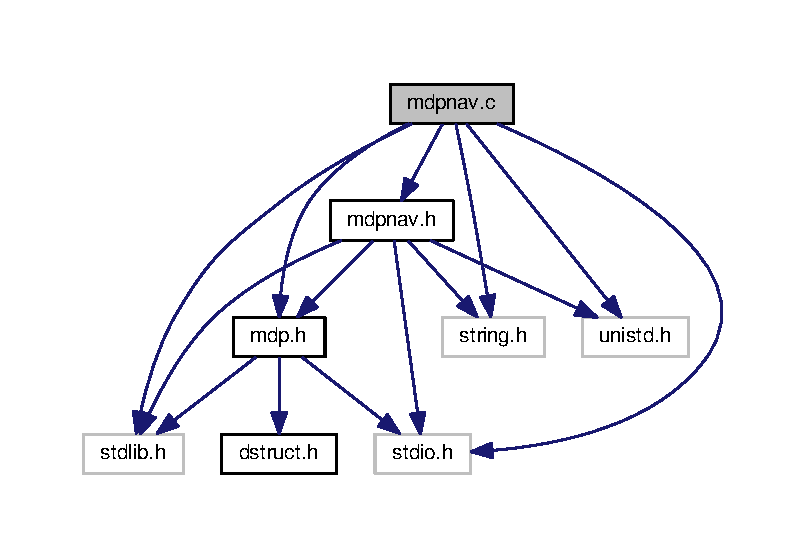
\includegraphics[width=350pt]{mdpnav_8c__incl}
\end{center}
\end{figure}
\subsection*{Functions}
\begin{DoxyCompactItemize}
\item 
void \hyperlink{mdpnav_8c_a2ce00cd6fdd1971fedd752da4dad1855}{report\+\_\+file} (\hyperlink{structmap}{map} $\ast$m, char $\ast$output\+\_\+file)
\begin{DoxyCompactList}\small\item\em writes the result to a file \end{DoxyCompactList}\item 
void \hyperlink{mdpnav_8c_a1016b889f9a188d71fe8dae4f83be7fb}{parse\+\_\+params} (int argc, char $\ast$argv\mbox{[}$\,$\mbox{]}, \hyperlink{structnav__spec}{nav\+\_\+spec} $\ast$p)
\begin{DoxyCompactList}\small\item\em parses command line arguments \end{DoxyCompactList}\item 
int {\bfseries main} (int argc, char $\ast$argv\mbox{[}$\,$\mbox{]})\hypertarget{mdpnav_8c_a0ddf1224851353fc92bfbff6f499fa97}{}\label{mdpnav_8c_a0ddf1224851353fc92bfbff6f499fa97}

\end{DoxyCompactItemize}


\subsection{Detailed Description}
Map Navigation with M\+D\+Ps. 

\begin{DoxyAuthor}{Author}
Stalin Muñoz Gutiérrez 
\end{DoxyAuthor}
\begin{DoxyDate}{Date}
3 March 2019 Basic Map Navigation with Markov Decision Processes 
\end{DoxyDate}


\subsection{Function Documentation}
\index{mdpnav.\+c@{mdpnav.\+c}!parse\+\_\+params@{parse\+\_\+params}}
\index{parse\+\_\+params@{parse\+\_\+params}!mdpnav.\+c@{mdpnav.\+c}}
\subsubsection[{\texorpdfstring{parse\+\_\+params(int argc, char $\ast$argv[], nav\+\_\+spec $\ast$p)}{parse_params(int argc, char *argv[], nav_spec *p)}}]{\setlength{\rightskip}{0pt plus 5cm}void parse\+\_\+params (
\begin{DoxyParamCaption}
\item[{int}]{argc, }
\item[{char $\ast$}]{argv\mbox{[}$\,$\mbox{]}, }
\item[{{\bf nav\+\_\+spec} $\ast$}]{p}
\end{DoxyParamCaption}
)}\hypertarget{mdpnav_8c_a1016b889f9a188d71fe8dae4f83be7fb}{}\label{mdpnav_8c_a1016b889f9a188d71fe8dae4f83be7fb}


parses command line arguments 


\begin{DoxyParams}{Parameters}
{\em argc} & number of command line arguments \\
\hline
{\em argv} & command line arguments \\
\hline
{\em p} & pointer to the parameter simulation structure \\
\hline
\end{DoxyParams}
\index{mdpnav.\+c@{mdpnav.\+c}!report\+\_\+file@{report\+\_\+file}}
\index{report\+\_\+file@{report\+\_\+file}!mdpnav.\+c@{mdpnav.\+c}}
\subsubsection[{\texorpdfstring{report\+\_\+file(map $\ast$m, char $\ast$output\+\_\+file)}{report_file(map *m, char *output_file)}}]{\setlength{\rightskip}{0pt plus 5cm}void report\+\_\+file (
\begin{DoxyParamCaption}
\item[{{\bf map} $\ast$}]{m, }
\item[{char $\ast$}]{output\+\_\+file}
\end{DoxyParamCaption}
)}\hypertarget{mdpnav_8c_a2ce00cd6fdd1971fedd752da4dad1855}{}\label{mdpnav_8c_a2ce00cd6fdd1971fedd752da4dad1855}


writes the result to a file 


\begin{DoxyParams}{Parameters}
{\em m} & the map of cells \\
\hline
{\em output\+\_\+file} & name of the output file \\
\hline
\end{DoxyParams}
\begin{DoxyReturn}{Returns}
the output is writen to the file 
\end{DoxyReturn}

\hypertarget{random__example_8c}{}\section{random\+\_\+example.\+c File Reference}
\label{random__example_8c}\index{random\+\_\+example.\+c@{random\+\_\+example.\+c}}


Example with a random instance of a 3 state \hyperlink{structMDP}{M\+DP}.  


{\ttfamily \#include $<$stdio.\+h$>$}\\*
{\ttfamily \#include \char`\"{}mdp.\+h\char`\"{}}\\*
Include dependency graph for random\+\_\+example.\+c\+:\nopagebreak
\begin{figure}[H]
\begin{center}
\leavevmode
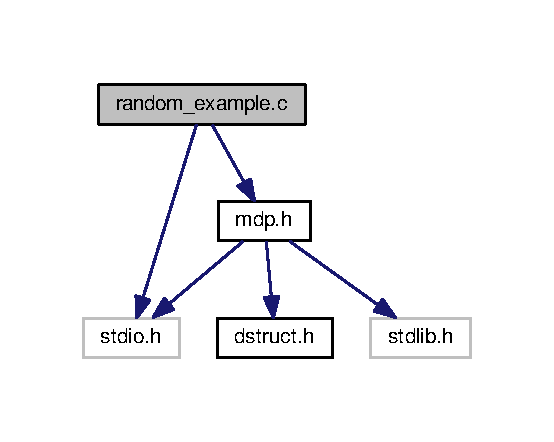
\includegraphics[width=266pt]{random__example_8c__incl}
\end{center}
\end{figure}
\subsection*{Functions}
\begin{DoxyCompactItemize}
\item 
void {\bfseries random\+\_\+example} ()\hypertarget{random__example_8c_a348f3d5bcb92f6284aedd25500adfe52}{}\label{random__example_8c_a348f3d5bcb92f6284aedd25500adfe52}

\item 
int \hyperlink{random__example_8c_a3c04138a5bfe5d72780bb7e82a18e627}{main} (int argc, char $\ast$$\ast$argv)
\begin{DoxyCompactList}\small\item\em Simple invocation of a random instance of an \hyperlink{structMDP}{M\+DP}. \end{DoxyCompactList}\end{DoxyCompactItemize}


\subsection{Detailed Description}
Example with a random instance of a 3 state \hyperlink{structMDP}{M\+DP}. 

\begin{DoxyAuthor}{Author}
Stalin Muñoz Gutiérrez 
\end{DoxyAuthor}
\begin{DoxyDate}{Date}
27 may 2018 
\end{DoxyDate}


\subsection{Function Documentation}
\index{random\+\_\+example.\+c@{random\+\_\+example.\+c}!main@{main}}
\index{main@{main}!random\+\_\+example.\+c@{random\+\_\+example.\+c}}
\subsubsection[{\texorpdfstring{main(int argc, char $\ast$$\ast$argv)}{main(int argc, char **argv)}}]{\setlength{\rightskip}{0pt plus 5cm}int main (
\begin{DoxyParamCaption}
\item[{int}]{argc, }
\item[{char $\ast$$\ast$}]{argv}
\end{DoxyParamCaption}
)}\hypertarget{random__example_8c_a3c04138a5bfe5d72780bb7e82a18e627}{}\label{random__example_8c_a3c04138a5bfe5d72780bb7e82a18e627}


Simple invocation of a random instance of an \hyperlink{structMDP}{M\+DP}. 


\begin{DoxyParams}{Parameters}
{\em argc} & number of command line params \\
\hline
{\em argv} & no params for this example \\
\hline
\end{DoxyParams}

\hypertarget{ryn__chapter__17_8c}{}\section{ryn\+\_\+chapter\+\_\+17.\+c File Reference}
\label{ryn__chapter__17_8c}\index{ryn\+\_\+chapter\+\_\+17.\+c@{ryn\+\_\+chapter\+\_\+17.\+c}}


Simple \hyperlink{structMDP}{M\+DP} library.  


{\ttfamily \#include $<$stdio.\+h$>$}\\*
{\ttfamily \#include $<$stdlib.\+h$>$}\\*
{\ttfamily \#include $<$time.\+h$>$}\\*
{\ttfamily \#include $<$double.\+h$>$}\\*
{\ttfamily \#include $<$math.\+h$>$}\\*
{\ttfamily \#include \char`\"{}mdp.\+h\char`\"{}}\\*
Include dependency graph for ryn\+\_\+chapter\+\_\+17.\+c\+:\nopagebreak
\begin{figure}[H]
\begin{center}
\leavevmode
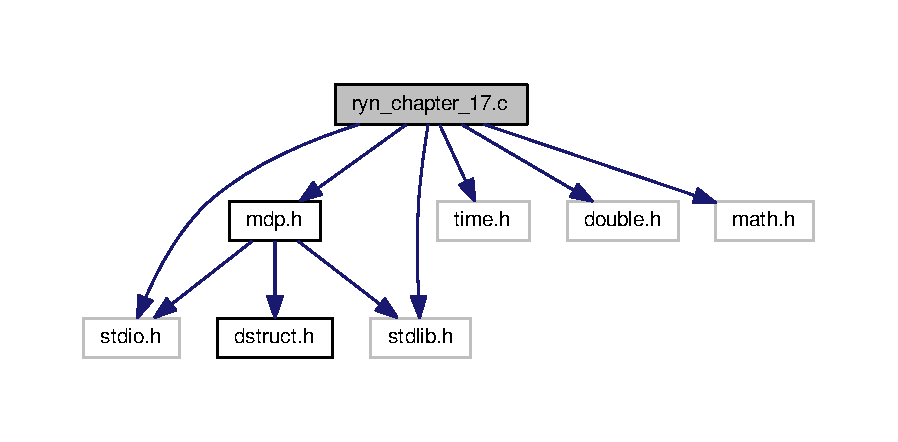
\includegraphics[width=350pt]{ryn__chapter__17_8c__incl}
\end{center}
\end{figure}
\subsection*{Functions}
\begin{DoxyCompactItemize}
\item 
void {\bfseries ryn\+\_\+chapter\+\_\+17} ()\hypertarget{ryn__chapter__17_8c_a480d17900073df58accbaec72b360e9a}{}\label{ryn__chapter__17_8c_a480d17900073df58accbaec72b360e9a}

\item 
int \hyperlink{ryn__chapter__17_8c_a3c04138a5bfe5d72780bb7e82a18e627}{main} (int argc, char $\ast$$\ast$argv)
\begin{DoxyCompactList}\small\item\em Runs the Russell \& Norvig chapter 17 example Russell, Stuart J., and Peter Norvig. Artificial intelligence\+: a modern approach. Pearson Education Limited, 2016. \end{DoxyCompactList}\end{DoxyCompactItemize}


\subsection{Detailed Description}
Simple \hyperlink{structMDP}{M\+DP} library. 

\begin{DoxyAuthor}{Author}
Stalin Muñoz Gutiérrez 
\end{DoxyAuthor}
\begin{DoxyDate}{Date}
28 may 2018 Simple Markov Decision Process library implementation. 
\end{DoxyDate}


\subsection{Function Documentation}
\index{ryn\+\_\+chapter\+\_\+17.\+c@{ryn\+\_\+chapter\+\_\+17.\+c}!main@{main}}
\index{main@{main}!ryn\+\_\+chapter\+\_\+17.\+c@{ryn\+\_\+chapter\+\_\+17.\+c}}
\subsubsection[{\texorpdfstring{main(int argc, char $\ast$$\ast$argv)}{main(int argc, char **argv)}}]{\setlength{\rightskip}{0pt plus 5cm}int main (
\begin{DoxyParamCaption}
\item[{int}]{argc, }
\item[{char $\ast$$\ast$}]{argv}
\end{DoxyParamCaption}
)}\hypertarget{ryn__chapter__17_8c_a3c04138a5bfe5d72780bb7e82a18e627}{}\label{ryn__chapter__17_8c_a3c04138a5bfe5d72780bb7e82a18e627}


Runs the Russell \& Norvig chapter 17 example Russell, Stuart J., and Peter Norvig. Artificial intelligence\+: a modern approach. Pearson Education Limited, 2016. 


\begin{DoxyParams}{Parameters}
{\em argc} & number of command line params \\
\hline
{\em argv} & no params for this example \\
\hline
\end{DoxyParams}

%--- End generated contents ---

% Index
\backmatter
\newpage
\phantomsection
\clearemptydoublepage
\addcontentsline{toc}{chapter}{Index}
\printindex

\end{document}
